%% This is an example first chapter.  You should put chapter/appendix that you
%% write into a separate file, and add a line \include{yourfilename} to
%% main.tex, where `yourfilename.tex' is the name of the chapter/appendix file.
%% You can process specific files by typing their names in at the 
%% \files=
%% prompt when you run the file main.tex through LaTeX.

\begingroup%
\makeatletter%
\cleardoublepage%
\let\newpage\relax%
\let\clearpage\relax%
\vspace*{\fill}%
\vspace*{\dimexpr-50\p@-\baselineskip}% Remove the initial
%% -default- 50pt gap (plus 1 line) 
\chapter{The Multiple Fates of Sinking Particles in the North Atlantic Ocean}
\label{chap2}
\let\thefootnote\relax\footnote{{\setlength{\parindent}{0pt}This chapter was originally published as:\\\\Collins, J. R., B. R. Edwards, K. Thamatrakoln, J. E. Ossolinski, G. R. DiTullio, K. D. Bidle, S. C. Doney, and B. A. S. Van Mooy. 2015. The multiple fates of sinking particles in the North Atlantic Ocean. \emph{Global Biogeochemical Cycles} \emph{29}:1471-1494; doi:\href{http://dx.doi.org/10.1002/2014GB005037}{10.1002/2014GB005037}\\\\\copyright 2015 American Geophysical Union}}
\vspace*{\fill}%
\endgroup%

\clearpage
\section{Abstract}
The direct respiration of sinking organic matter by attached bacteria is often invoked as the dominant sink for settling particles in the mesopelagic ocean. However, other processes, such as enzymatic solubilization\textsuperscript{1}\let\thefootnote\relax\footnote{{\setlength{\parindent}{0pt}\textsuperscript{1} i.e., via exoenzyme hydrolysis. The term ``enzymatic solubilization'' is used throughout the chapter.}} and mechanical disaggregation, also contribute to particle flux attenuation by transferring organic matter to the water column. Here we use observations from the North Atlantic Ocean, coupled to sensitivity analyses of a simple model, to assess the relative importance of particle-attached microbial respiration compared to the other processes that can degrade sinking particles. The observed carbon fluxes, bacterial production rates, and respiration by water column and particle-attached microbial communities each spanned more than an order of magnitude. Rates of substrate-specific respiration on sinking particle material ranged from 0.007 $\pm$ 0.003 to 0.173 $\pm$ 0.105 day\textsuperscript{-1}. A comparison of these substrate-specific respiration rates with model results suggested sinking particle material was transferred to the water column by various biological and mechanical processes nearly 3.5 times as fast as it was directly respired. This finding, coupled with strong metabolic demand imposed by measurements of water column respiration (729.3 $\pm$ 266.0 mg C m\textsuperscript{-2} d\textsuperscript{-1}, on average, over the 50 to 150 m depth interval), suggested a large fraction of the organic matter evolved from sinking particles ultimately met its fate through subsequent remineralization in the water column. At three sites, we also measured very low bacterial growth efficiencies and large discrepancies between depth-integrated mesopelagic respiration and carbon inputs.
\clearpage
\section{Introduction}
The efficiency of the ocean's biological pump, one of the two primary mechanisms by which carbon dioxide is chemically reduced and exported to depth, is defined by a fine balance between primary production in the marine surface layer and the destruction of this organic matter in and below the euphotic zone. The majority of this export occurs as a rain of sinking particles that are progressively remineralized by heterotrophic bacteria or zooplankton as they sink through the mesopelagic ocean (Buesseler and Boyd, 2009; Buesseler et al., 2007b; Steinberg et al., 2008b). Respiration by particle-associated heterotrophic communities has been invoked in several specific ecosystems as the primary sink for these particles, based on observations either in the field or in the laboratory (e.g., McDonnell et al., 2015; Ploug et al., 1999) or statistical relationships, for example, between the remineralization length scale and temperature (Marsay et al., 2015). However, modeling exercises, together with an increasing number of environmental studies, indicate that a substantial fraction of particles from the ocean's surface can be degraded during their downward transit by other processes that rival particle-attached microbial respiration in magnitude (Close et al., 2013; Giering et al., 2014; Ki\o{}rboe, 2001; Ki\o{}rboe and Jackson, 2001; Stemmann et al., 2004a, 2004b; Taylor and Karl, 1991).

Observational and experimental evidence both suggest that particle disaggregation and solubilization can transfer sinking organic matter to the suspended particulate (POM\textsubscript{susp}) or dissolved organic matter (DOM) pools, as an alternative to direct respiration (Alldredge, 2000; Grossart and Simon, 1998; Smith et al., 1992). The POM\textsubscript{susp} and DOM can then provide an immediate metabolic substrate for free-living bacteria in the water column (Ki\o{}rboe and Jackson, 2001). Alternatively, dissolved organic matter can remain within the 662 Pg pool of marine dissolved organic carbon (DOC), where it may be later respired or instead removed by some other process (Azam, 1998; Hansell et al., 2009). Zooplankton can serve both as a sink for particle material, via respiration or mechanical disaggregation, and as a source of particles below the mixed layer. At depth, zooplankton can egest fecal pellets following their daily vertical migration from the ocean's surface (Steinberg et al., 2008b); they may also ``repackage'' suspended particles at depth into sinking particles.

Establishing the relative contributions of these various particle degradation processes to total observed particle flux attenuation remains a principal challenge in investigations of the marine carbon cycle, particularly at global and basin scales (Burd et al., 2010; Sanders et al., 2014; Siegel et al., 2014). The inability to accurately, precisely, and reliably quantify the relative importance of these processes has been identified as a significant source of uncertainty in continuing efforts to ascertain the metabolic state of various ocean ecosystems (Buesseler and Boyd, 2009; Ducklow and Doney, 2013). Many of these studies have identified order-of-magnitude imbalances in the mesopelagic and upper bathypelagic between inputs of settling organic matter and metabolic sinks, often with large uncertainties attached to the latter (del Giorgio et al., 1997; Duarte et al., 2013; Geider, 1997; Williams and Robertson, 1991; Reinthaler et al., 2006; Steinberg et al., 2008b). Even in the few recent studies that have narrowed or closed this mass imbalance, authors have relied on literature surveys, models, or significant interpolation for many of the sink terms associated with bacterial respiration and particle flux attenuation (Aranguren-Gassis et al., 2012; Giering et al., 2014; Westberry et al., 2012).

\begin{figure}[!p]
\centering
\includegraphics[width=0.75\textwidth]{Fig_2-1.pdf}
\captionsetup{font={footnotesize}}
\caption[Schematic showing the major processes that ultimately remove sinking particle material in the mesopelagic ocean, as conceptualized in \autoref{chap2}.]{Schematic showing the major processes that ultimately remove sinking particle material in the mesopelagic ocean, as conceptualized in \autoref{chap2} of the thesis (Collins et al., 2015). Also shown are the accompanying first-order rate constants ($k$; units of day$^{-1}$) through which we represent these attenuation processes in the model described in that chapter. Arrow a, in magenta: Respiration of particle material by particle-attached heterotrophic bacteria ($k_{R}$, which we calculate from direct measurements). We use a single rate constant ($k_{S,D,Z}$) in our model sensitivity analyses to account for the other processes (arrows b-e), which we did not directly observe. $k_{S,D,Z}$ represents the fraction of particle flux attenuation that cannot be attributed to direct respiration by particle-attached bacteria. Arrow b, in orange: Enzymatic solubilization or mechanical disaggregation of particle material by attached bacteria. This process transfers organic matter to the dissolved or suspended (i.e., colloidal) phases in the surrounding water column, where it can then be metabolized by free-living bacterial communities (arrows f and g). Arrows c-e, in green: Particle flux attenuation processes attributable to zooplankton, including (arrow c) mechanical disaggregation (e.g., ``sloppy feeding''), (arrow d) egestion or excretion, or (arrow e) direct respiration of material to carbon dioxide. Disaggregation and excretion can transfer particle material to the dissolved or suspended (i.e., colloidal) phases; egestion of smaller fecal pellets can also transfer material to the suspended organic matter pool. Our interpretation of the sensitivity analysis results was informed by additional direct observations of arrow g.}
\label{fig:c2n1}
\end{figure}

Here we sought to determine the relative contribution to particle flux attenuation by respiration compared to the other major biological and mechanical processes that progressively remove sinking particles with depth (\autoref{fig:c2n1}). While we focus in this study on the ultimate mass-balance sinks for these particles, complex mechanisms act to both disaggregate and re-aggregate particles continuously as they sink through the water column (Burd, 2013; Jackson and Burd, 1998). In this study, we first present measurements collected at six stations in North Atlantic basin (\autoref{fig:c2n2}) of sinking particulate carbon fluxes, water column bacterial production and respiration rates, and specific respiration rates on sinking particle material. From these data, we calculate substrate-specific respiration rates on sinking particles, bacterial growth efficiencies (\emph{BGE}) both in the water column and on sinking particle material, and depth-integrated estimates of water column BP and respiration for the upper mesopelagic zone (50 to 150 m). We then use our measurements of particulate organic carbon (POC) fluxes and substrate-specific respiration in a series of sensitivity analyses of a simple, yet mechanistic model of particle flux attenuation. Model-observed deviations allow us to place a minimum constraint at each station on the average particle sinking velocity, \emph{W\textsubscript{avg}}. We then combine our observational data and the results of these sensitivity analyses to (1) constrain the relative contribution to particle flux attenuation by particle-attached microbial respiration compared to other processes and (2) determine how differences in \emph{W\textsubscript{avg}} affect this partitioning. Our objective in quantifying this partitioning was to inform how respiration and other particle flux attenuation processes should be prioritized and parameterized in new models of marine carbon export (e.g., Siegel et al., 2014).

\section{Methods and Model Description}

\subsection{Cruises and Study Locations}


Conductivity-temperature-depth (CTD) data and water samples were collected on two cruises aboard the R/V \emph{Knorr} in 2012: BLATZ II (KN207-1; \url{http://www.bco-dmo.org/deployment/58787}) and NA VICE (KN207-3; \url{http://www.bco-dmo.org/project/2136}). The cruise tracks (\autoref{fig:c2n2}) allowed us to capture data for a variety of biogeographical provinces (Longhurst, 2010) in the North Atlantic Ocean over the course of 4 months. Deployments of sediment traps and shipboard incubations for determination of respiration rates in water column and sinking particle samples were performed during both cruises at six, 3 to 5 day, quasi-Lagrangian process stations. In addition, the rate of bacterial production was measured at each process station and along both cruise tracks. Process station locations were chosen based on physical and biological properties determined from real-time sea surface height and ocean color remote sensing data. Station PS-3 was reoccupied after approximately one week as station PS-4.

\subsection{Sediment Trap Deployments}

Vertically sinking particulate carbon fluxes were measured at 50, 150, and 300 m using surface-tethered cylindrical sediment traps (0.0125 m\textsuperscript{2} cross-sectional area; materials and construction as described in McDonnell and Buesseler (2012)). A mooring consisting of four traps at each depth, a surface buoy, wave-action mitigation bungee cord, and several floats, was deployed at each process station and allowed to drift for 3-5 days. The quasi-Lagrangian behavior of the mooring during each deployment was confirmed by comparison of positional data obtained from an Argos satellite beacon mounted on the surface buoy with shipboard acoustic Doppler current profiler data from the R/V \emph{Knorr}, which trailed the mooring at a range of 1-2 miles.

Traps were prepared, deployed, and recovered as described in McDonnell and Buesseler (2012). Traps were then sampled for particulate carbon in accordance with McDonnell and Buesseler (2012), except that the screened brine suspension (350 $\mu$m pore size, to exclude macrozooplankton) was filtered onto a series of precombusted, 47 mm GF/F filters (0.7 $\mu$m nominal pore size). Field and analytical blanks were collected at each station. Filters were immediately frozen in liquid nitrogen and then stored at -80$^{\circ}$C.

\subsection{Determination of Particulate Carbon Fluxes}

Filters from three of the four traps at each depth were used for determination of total particulate and particulate inorganic carbon (TPC and PIC, respectively). After thawing, the filters (including blanks) were first dried at 70$^{\circ}$C in a drying oven; each filter was then weighed and cut in half with precombusted stainless steel scissors. Each half was then weighed separately. One half was reserved for PIC analysis and the other reserved for determination of TPC. For TPC, sets of filter halves were transferred to 12 mm by 20 cm precombusted quartz tubes containing copper oxide (100 mg) and elemental silver wires. The tubes were then attached to a vacuum line, evacuated, flame-sealed, and combusted at 850$^{\circ}$C for 10 h. The evolved carbon dioxide was then isolated through a series of cold traps and quantified manometrically. PIC was determined from the other set of filter halves by coulometric analysis of acidified samples using a Model CM5014 UIC Coulometric Analyzer with Carbonate Acidification Module, as described in Honjo et al. (1995). Particulate organic carbon (POC) was determined for each trap by difference of the blank-corrected TPC and PIC measurements. An instrument failure in the laboratory prevented us from analyzing particle flux samples from station PS-1.

\subsection{Bacterial Production}

Water column bacterial production (BP) rates were measured at each process station and along both cruise tracks using the \textsuperscript{3}H-leucine incorporation microcentrifuge method of Simon and Azam (1989), as modified by Kirchman (2001). Incubations were conducted following each CTD cast using water samples from six depths; the first and sixth samples were always from the immediate surface layer (3-5 m) and 150 m. In addition, at process stations QL-1 and QL-2 (both on the eastern cruise leg), we conducted incubations for BP using sinking particle material retrieved from large-diameter net traps (see \autoref{ssec:Respiration by Bacteria Attached to Sinking Particles} below). Triplicate 1 mL samples from each chosen depth or net trap were incubated with \textsuperscript{3}H-leucine (PerkinElmer, Inc., Waltham, MA; 146.5 Ci mmol\textsuperscript{-1}, diluted to achieve 20 nM final concentration) for 4-12 h. Limited incubator space available for radiotracer work on the two cruises required us to incubate all BP samples from a given station at the same temperature. We chose a temperature that was most representative of the temperatures at the depths from which the majority of samples were drawn; this was, in almost all cases, the temperature of the mixed layer. Incubation of deeper samples (e.g., from 150 m) at this temperature could in some cases have biased the observed rates. However, we suspect such a temperature bias would only have been consequential at stations PS-2, PS-3, and PS-4, which were characterized by a significant vertical temperature gradient; at the other stations, the vertical temperature gradient did not exceed 3$^{\circ}$C (\autoref{fig:c2n3}e).

\begin{SCfigure}[0.5][!bh]
\centering
\includegraphics[width=0.6\textwidth]{Fig_2-2.pdf}
\captionsetup{font={footnotesize}}
\caption[Cruise tracks and sampling locations referenced in \autoref{chap2}.]{(a) Cruise tracks (blue, KN207-1 and red, KN207-3) and locations in the North Atlantic basin of the quasi-Lagrangian stations at which we conducted 3-5 day deployments of surface-tethered sediment traps and made measurements of respiration and bacterial production on sinking particle material. Symbols representing the locations of the six stations correspond to the data plotted in \autoref{fig:c2n3} and \autoref{fig:c2n4}. (b) Map expansion, showing locations of stations PS-3 and PS-4 superimposed over 8 day average MODIS Aqua surface reflectance at 555 nm. This parameter is an indicator of PIC concentration.}
\label{fig:c2n2}
\end{SCfigure}

At the conclusion of the two cruises, samples were processed and analyzed in a laboratory ashore according to Kirchman (2001) using Ultima Gold Low-Level Tritium cocktail (PerkinElmer, Inc.). Decay per minute counts in killed control samples were subtracted from the mean of each set of triplicates and divided by the incubation time to obtain a blank-corrected leucine incorporation rate (\emph{leu\textsubscript{inc}}) in units of pmol leucine L\textsuperscript{-1} h\textsuperscript{-1}.

To convert our volumetric measurements of \emph{leu\textsubscript{inc}} to carbon-based estimates of bacterial production (BP), we applied the basic equation
\begin{equation} \label{eq:c2e1}
BP = {\nu _{C:leu}}le{u_{inc}}ID
\end{equation}
where $\nu _{C:leu}$ $\nu _{C:leu}$ is a theoretical or empirical carbon to leucine conversion factor and \emph{ID} is a scaling factor that accounts for isotope dilution, i.e., the degree to which the added \textsuperscript{3}H-leucine was diluted within the cell by endogenous leucine sources. We employed two strategies with regard to the values of the scaling factors. First, to obtain individual estimates of water column and particle-attached bacterial production (\emph{BP\textsubscript{wc}} and \emph{BP\textsubscript{pa}}, respectively) in units of mg C m\textsuperscript{-3} d\textsuperscript{-1}, we applied a constant $\nu _{C:leu}$ of 1.5 kg C (mol leucine)\textsuperscript{-1} (Kirchman, 2001; Simon and Azam, 1989) and made the conservative assumption that \emph{ID} \emph{=}  1, i.e., that bacteria in our incubations had satisfied their leucine demand using only the added radiolabeled substrate. These are the results we report in \autoref{table:c2n2} and use for the upper axes in \autoref{fig:c2n3} and \autoref{fig:acn2} in the supporting information.

However, empirical evidence indicates that $\nu _{C:leu}$ and \emph{ID} both can vary considerably in the environment across depth, space, and time. \emph{ID} is difficult to measure and can represent a significant source of uncertainty in calculations of bacterial production (Chin-Leo and Kirchman, 1988; Ducklow and Hill, 1985; Kirchman, 2001). While variation in $\nu _{C:leu}$ is often more amenable to prediction (e.g., according to \emph{BGE}) (Alonso-Saez et al., 2008), it too varies widely (Giering et al., 2014). Therefore, as a second strategy, we used a bootstrap Monte Carlo analysis to consider wide variation in both of these parameters in our estimates of depth-integrated bacterial production, \emph{BP\textsubscript{int}}, from 50 to 150 m.

To obtain our estimates of \emph{BP\textsubscript{int}}, we followed the method of Giering et al. (2014), using the observational uncertainties in our water column measurements of \emph{leu\textsubscript{inc}} (\emph{N}  = 6 per station, as above) to fit a series of 100,000 bootstrap power law distributions to the data at each station, in increments of 0.1 m. A power law distribution provided the best empirical fit to the data from a range of simple functions we considered (\autoref{fig:c2n3}c). We then numerically integrated the bootstrap samples in each simulated data set from 50 to 150 m, according to
\begin{equation} \label{eq:c2e2}
B{P_{int}} = \int\limits_{z = 50}^{150} {le{u_{inc}}{\nu _{C:leu}}IDdz}
\end{equation}
In each simulation, we allowed \emph{ID} to take any value from 1 to 2, assuming a uniform distribution between the two extremes. We allowed $\nu _{C:leu}$ to vary according to a set of empirical values assembled from the literature by Giering et al. (2014) for depths \textgreater{} 50 m, which we assumed were normally distributed (\emph{N} = 21; mean $\pm$ standard deviation, 0.44 $\pm$ 0.27 kg C (mol leucine)\textsuperscript{-1}). We then used the mean and standard deviation of these repeated integrations to estimate a central value and uncertainty for \emph{BP\textsubscript{int}} at each station. This method allowed us to obtain estimates (\autoref{table:c2n3}) that reflected both observational uncertainties and possible variation in the two scaling factors.

\subsection{Photosynthetic Pigments}
\label{sec:Photosynthetic Pigments}

To evaluate the taxonomic composition of the phytoplankton community at each station, analysis of photosynthetic pigments was performed by high-performance liquid chromatography (HPLC). At each process station, water samples were collected from multiple depths via shipboard CTD and filtered onto precombusted 0.7 $\mu$m glass fiber filters. HPLC analysis was conducted in the laboratory according to DiTullio and Geesey (2003).

\subsubsection{Remote Sensing Data Analysis}

To generate the image in \autoref{fig:c2n1}b, we used 8-day average, level 3 MODIS AQUA satellite data of surface reflectance at 555 nm. A 4 km resolution data file (A201217720\\12184.L3m\_8D\_RRS\_Rrs\_555\_4km.hdf) was retrieved using the NASA GSFC\\OceanColor Level 3 Browser at \url{http://oceancolor.gsfc.nasa.gov/cgi/l3}. The false-color image was generated in ArcGIS 10.1 after geographical indexing.

\subsection{Respiration Measurements}

\subsubsection{Water Column Respiration}

Estimates of aerobic respiration by the water column microbial community (\emph{WCR}) were calculated by linear regression of measurements of dissolved oxygen concentration in a series of 300 mL shipboard bottle incubations. We made profiles of water column respiration at stations PS-2, PS-3, and PS-4; we made only one water column respiration measurement, in the euphotic zone, at each of the three other stations (QL-1, QL-2, and PS-1). Determination of dissolved oxygen was made at 3 to 9 h intervals in at least five replicates using optode spot minisensors (PreSens PSt3; Precision Sensing GmbH, Regensburg, Germany) that were glued to the inside surfaces of the bottles using food quality silicone cement (Warkentin et al., 2007). The use of these optode spots eliminated the need for drawing of aliquots from the sample bottles. Incubations were conducted in the dark at in situ temperature as described in Edwards et al. (2011). We validated the rates from these incubations using a series of Winkler titrations; methods are described in the supporting information. We used the standard error of the slope parameter from these regressions as the uncertainty in our estimates of \emph{WCR}. Depth-integrated water column respiration (\emph{WCR}\textsubscript{int}) was calculated from water column observations at stations PS-2, PS-3, and PS-4 (\emph{N} = 9, 6, and 7, respectively) using the same 100,000 simulation bootstrap method as for \emph{BP\textsubscript{int}}.

\subsubsection{Respiration by Bacteria Attached to Sinking Particles}
\label{ssec:Respiration by Bacteria Attached to Sinking Particles}

For determination of respiration by bacteria attached to sinking particles, particulate material was collected from the appropriate depth using a series of surface-tethered, large-diameter net traps with a detachable 0.2 $\mu$m mesh cod end (Peterson et al., 2005). These traps were allowed to drift from a surface mooring for approximately 24 h in the same eddy feature as the corresponding cylindrical sediment traps. The exact deployment time was controlled by use of a remote acoustic release, which allowed us to close the traps prior to recovery.
Upon recovery, the particle material in the cod end was homogenized by gentle shaking, then quantitatively split into fractions using an eight-way rotating electric splitter (Lamborg et al., 2008); aliquots were taken from one or more of these fractions, screened to 350 $\mu$m to exclude larger mesozooplankton, and dispensed quantitatively into replicate biochemical oxygen demand (BOD) bottles for incubation. The 350 $\mu$m screen was inspected to ensure it had not retained any particle material. Incubation bottles were then made up to volume with seawater retrieved by CTD cast from the same depth as the trap, and oxygen concentrations were monitored over time using optode sensor spots, as described above. An additional quantitative split was immediately collected by vacuum onto a precombusted 0.7 $\mu$m GF/F filter for determination of POC. POC was determined for these samples from the preserved filter by elemental analyzer (Carlo Erba Model 1108) after acid-fuming to remove the inorganic carbon fraction.

A substrate-specific respiration rate (\emph{k\textsubscript{R}}\textsubscript{;} units of mol C\textsubscript{respired}:mol POC d\textsuperscript{-1}) was determined from these measurements according to an adaptation of McDonnell (2011):
\begin{equation} \label{eq:c2e3}
{k_R} = \frac{{({r_{pa}} - {r_{col}}){V_{inc}}{\nu _{{\text{C:}}{{\text{O}}_{\text{2}}}}}}}{{PO{C_{trap}}}}
\end{equation}
where \emph{r\textsubscript{pa}} and \emph{r\textsubscript{col}} are volumetric respiration rates from the particle-attached and water column samples, respectively, calculated by simple linear regression from replicate shipboard incubations; \emph{V\textsubscript{inc}} is the incubation volume (300 mL); \emph{POC\textsubscript{trap}} is the quantity of POC used in the incubation; and $\nu _{{\text{C:}}{{\text{O}}_{\text{2}}}}$ is a molar respiratory quotient for the remineralization of organic matter at depth (we applied a value of 117/170) (Anderson and Sarmiento, 1994).

\subsubsection{Use of Winkler Titrations to Validate Respiration Rate Calculations}

To validate the water-column respiration rates we derived from our shipboard incubations, we used a simple method based on a series Winkler titrations. Winkler titration remains the standard analytical method for determination of dissolved oxygen in water (EPA Method 360.2 as modified for shipboard determination in seawater; U S EPA, 1983). For the comparison, we chose the depth in each respiration profile (\autoref{fig:c2n3}) that corresponded to the middle of the mixed layer (\autoref{table:c2n3}). We determined the respiration rate at this depth using triplicate samples sacrificed at two timepoints. A \emph{t} = 0 dissolved oxygen concentration was determined immediately in samples collected from the same CTD cast used for the respiration profile. A final concentration was determined using 300 mL samples that had been incubated alongside the optode sensor spot bottles. The respiration rate was determined by simple difference of the mean concentrations at the two timepoints.

\subsection{Bacterial Growth Efficiency}

Bacterial growth efficiency (\emph{BGE}) is a fundamental constraint on both bacterial growth and on microbial food web pathways that consume secondary production. It can be defined generally as the balance between bacterial production and bacterial respiration (BR) or
\begin{equation} \label{eq:c2e4}
BGE = \frac{{BP}}{{BP + BR}}
\end{equation}
We used our observations of \emph{BP\textsubscript{wc}} and \emph{WCR} to calculate the water column bacterial growth efficiency (\emph{BGE\textsubscript{wc}}) for depths \textgreater{} 50 m at stations PS-2, PS-3, and PS-4. We assumed in these calculations that, at these depths, our measurements of \emph{WCR = BR}; i.e., that no other microbiota (algae, protists, nanozooplankton, etc.) contributed to the oxygen consumption we observed in our incubations. We discuss the implications of this assumption for our results in \autoref{sssec:Enigmatically Low Efficiencies of Bacterial Growth}. We also calculated the growth efficiency on sinking particle material (\emph{BGE\textsubscript{pa}}) at stations QL-1 and QL-2, where we had observations of both particle-attached \emph{BP} and \emph{BR}.

\subsection{Sensitivity Analyses of a Simple Yet Mechanistic Flux Attenuation Model}

To complement our observations, we used sensitivity analyses of a simple model to diagnose the relative contributions to particle flux attenuation by direct respiration compared to other degradation processes. We also used these sensitivity analyses to place a minimum constraint on \emph{W\textsubscript{avg}} at each station. Models of particle flux attenuation range from the purely empirical, including the classic power law Martin curve, in which the exponent \emph{b} does not represent any particular thermodynamic process but can be used for comparison across ecosystems (Buesseler et al., 2007b; Martin et al., 1987), to models that attempt to account explicitly for the many complex mechanisms that form, destroy, and alter sinking particles (Anderson and Tang, 2010; Stemmann et al., 2004a).

\subsubsection{Model Specification}

Because our objective was to estimate generally the contribution to POC flux attenuation by particle-attached bacterial respiration compared to other possible processes, we chose to modify a simple, mechanistic, and frequently invoked exponential model of sinking particle flux attenuation that uses as primary inputs (1) sediment trap derived-particle fluxes and (2) rates of specific respiration on sinking particles (\emph{k\textsubscript{R}}; day\textsuperscript{-1}) (Boyd and Trull, 2007; Buesseler and Boyd, 2009; Lutz et al., 2002; McDonnell et al., 2015; Sarmiento and Gruber, 2006; Volk and Hoffert, 1985). In the model, the POC flux at a given depth \emph{z} (\emph{F\textsubscript{z}}, in mg C m\textsuperscript{-2} d\textsuperscript{-1}) is proportional to the flux observed at an overlying depth (\emph{F}\textsubscript{0}), which is attenuated according to first-order kinetics over a characteristic remineralization length scale (\emph{L\textsubscript{remin}}):
\begin{equation} \label{eq:c2e5}
{F_z} = {F_0}{e^{ - (z - {z_0})/{L_{remin}}}}
\end{equation}
A full derivation of \autoref{eq:c2e5} can be found in Sarmiento and Gruber (2006). We defined the length scale \emph{L\textsubscript{remin}} as the quotient of \emph{W\textsubscript{avg}} and the sum of two first-order rate constants that represent mechanistically, according to first-order kinetics, the processes (\autoref{fig:c2n1}) through which we assumed sinking POC could be oxidized or lost to the surrounding water column:
\begin{equation} \label{eq:c2e6}
{L_{remin}} = \frac{{{W_{avg}}}}{{{k_R} + {k_{S,D,Z}}}}
\end{equation}
\emph{k\textsubscript{R}} (day\textsuperscript{-1}) is the rate of oxidation of sinking POC by particle-attached bacteria, which we calculate from observations. \emph{k\textsubscript{S}}\textsubscript{,\emph{D},\emph{Z}} is a parameter of unknown magnitude that we use to estimate the rate of degradation of sinking POC by other processes; we diagnose the value of \emph{k\textsubscript{S}}\textsubscript{,\emph{D},\emph{Z}} using our sensitivity analyses to make comparisons with \emph{k\textsubscript{R}}.

In our conceptualization (\autoref{fig:c2n1}), the particle flux attenuation processes captured in \emph{k\textsubscript{S}}\textsubscript{,\emph{D},\emph{Z}} include (1) enzymatic solubilization (Azam and Malfatti, 2007) and (2) mechanical disaggregation, which transfer of sinking POC to the water column as dissolved organic carbon (DOC) or suspended POC (POC\textsubscript{susp}), and (3) various activities of zooplankton (discussed below). Solubilization occurs primarily via the activity of ectohydrolytic enzymes associated with bacterial cells, but can also be abiotic in origin (Taylor and Karl, 1991). Because ectoenzymes have high specificities for the different chemical components of sinking particle material, their relative contribution to disaggregation and dissolution will depend on how well the respective enzyme pool matches particle composition (Azam and Malfatti, 2007). Zooplankton can attenuate fluxes of sinking POC via mechanical disaggregation (e.g., ``sloppy feeding'' or ``zooplankton mining''), egestion or excretion or direct respiration. Shear stresses in the turbulent mixed layer are often strong enough to induce abiotic disaggregation of sinking particles, but evidence suggests abiotic shear does not play a major role in disaggregation in the ``quiescent'' mesopelagic ocean (Alldredge et al., 1990; Stemmann et al., 2004a). Although we do not consider mid-water shear in our conceptualization of particle flux attenuation, its effect would be captured in \emph{k\textsubscript{S}}\textsubscript{,\emph{D},\emph{Z}}.

Our definition of \emph{L\textsubscript{remin}} thus differs from previous parameterizations (e.g., McDonnell et al., 2015) by accounting in \emph{k\textsubscript{S}}\textsubscript{,\emph{D},\emph{Z}} for the losses of sinking particulate carbon to processes distinct from particle-attached bacterial respiration. Our parameterization does not allow us to further partition flux attenuation among these other processes (as in, e.g., Stemmann et al. (2004a)); however, our primary objective was only to estimate their collective strength compared to respiration by particle-attached bacteria. In addition, because we limited \autoref{eq:c2e5} and \autoref{eq:c2e6} to include a relatively small number of terms, we were required to diagnose or assume the values of only two unmeasured parameters, \emph{k\textsubscript{S}}\textsubscript{,\emph{D},\emph{Z}} and \emph{W\textsubscript{avg}}.

In applying \autoref{eq:c2e5} to sinking POC fluxes measured with surface-tethered sediment traps, we made several assumptions about the various biases inherent in the collection method. Horizontal shear can reduce the quantity of certain fractions of organic matter captured in moored traps relative to neutrally buoyant sediment traps or other collection methods (Stanley et al., 2004). Although there is evidence that the horizontal flow field can vary considerably across the depth range over which we made our measurements (Buesseler et al., 2007a), we assumed that any horizontal flow acted equally on the traps deployed at the three different depths, thus introducing a uniform bias for a given study site. We also assumed that the increase in the volume of ocean integrated by the traps at each successive depth (i.e., the ``statistical funnel'') (e.g., Siegel et al., 2008) was not so significant as to invalidate the use of measurements from different depths in the same model.

\subsubsection{Model Sensitivity Analyses and Bootstrap Monte Carlo Simulation}

We performed sensitivity analyses of the model over two depth intervals at five of our six stations (50-150 m and 150--300 m at QL-1, QL-2, PS-2, PS-3, and PS-4, yielding 10 observations of particle flux attenuation). Since we were able to fix the value of \emph{k\textsubscript{R}} at each station based on our observations, we used the sensitivity analyses to compute \emph{L\textsubscript{remin}} over a range of possible values for and \emph{k\textsubscript{S}}\textsubscript{,\emph{D},\emph{Z}}. We considered a range of values for \emph{W\textsubscript{avg}} (from 1 to 200 m d\textsuperscript{-1}, in 0.1 m d\textsuperscript{-1} increments) that encompassed those in the published literature for the temperate North Atlantic Ocean at depths \textless{} 1000 m; the results of our literature review are assembled in \autoref{table:acn1}. For \emph{k\textsubscript{S}}\textsubscript{,\emph{D},\emph{Z}}, we considered 1000 logarithmically distributed values from 10\textsuperscript{-5} d\textsuperscript{-1} (implying effectively no flux attenuation due to processes other than particle-attached bacterial respiration) to 1 day\textsuperscript{-1}, spanning several orders of magnitude and broadly encompassing our observed values of \emph{k\textsubscript{R}}. Because \emph{k\textsubscript{S}}\textsubscript{,\emph{D},\emph{Z}} was a parameter we created here to achieve our study objective, we found no truly equivalent values for it in the literature. At each station and depth interval, we then used the observational uncertainties in the inputs \emph{k\textsubscript{R}} and \emph{F}\textsubscript{0} to generate from \autoref{eq:c2e5} and \autoref{eq:c2e6} a simulated bootstrap data set of predictions of \emph{F\textsubscript{z}} (\emph{N} = 100,000) for each different pair of values of \emph{k\textsubscript{S}}\textsubscript{,\emph{D},\emph{Z}} and \emph{W\textsubscript{avg}}. We took the mean and standard deviation of each set of predictions to estimate the model flux (\emph{F\textsubscript{z}\textsubscript{,mod}}) and accompanying uncertainty ($\sigma_{mod}$) for each combination of \emph{k\textsubscript{S}}\textsubscript{,\emph{D},\emph{Z}} and \emph{W\textsubscript{avg}}.
ZXa
We then compared each model prediction (\emph{N} = $2\times10^6$ possible combinations per depth interval) to the observed flux at that station and depth (\emph{F\textsubscript{z}\textsubscript{,obs}}) using a simple measure of model-observed deviation (${F_{z,mod}} - {F_{z,obs}}$). Variation in this parameter at each station allowed us to diagnose the model's sensitivity to changes in \emph{k\textsubscript{S}}\textsubscript{,\emph{D},\emph{Z}} and \emph{W\textsubscript{avg}}. To determine whether the model-observed deviation was statistically significant, we tested the null hypothesis
\begin{equation} \label{eq:c2e7}
{H_0}:{F_{z,mod}} - {F_{z,obs}} = 0
\end{equation} 
at the $1\sigma$ confidence level. We rejected \emph{H}\textsubscript{0} where the absolute value of the model-observed deviation was greater than or equal to the root sum of the squared uncertainties or
\begin{equation} \label{eq:c2e8}
\left| {{F_{z,mod}} - {F_{z,obs}}} \right| \geq \sqrt {\sigma _{mod}^2 + \sigma _{obs}^2}
\end{equation} 
We used this test to assess a $1\sigma$ confidence region on the sensitivity analysis results at each station. We then excluded from further consideration those values of \emph{W\textsubscript{avg}} and \emph{k\textsubscript{S}}\textsubscript{,\emph{D},\emph{Z}} for which the model-observed deviation lay outside this region.

\section{Results and Discussion of Field Observations}

\subsection{POC and PIC Export}

Sinking particulate carbon fluxes captured with sediment traps varied geographically according to biogeochemical province and the composition of the phytoplankton community responsible for the majority of carbon fixation at each station (\autoref{fig:c2n3} and \autoref{table:c2n2}). POC fluxes at 50 m ranged from 47.9 $\pm$ 16.5 to 249 $\pm$ 16.3 mg C m\textsuperscript{-2} d\textsuperscript{-1}, while fluxes at 150 m ranged from 25.2 $\pm$ 2.0 to 208 $\pm$ 16.5 mg C m\textsuperscript{-2} d\textsuperscript{-1}. We observed the greatest variation in sinking carbon flux at 300 m; POC fluxes at that depth varied by a factor of 14, ranging from 9.6 $\pm$ 0.9 to 14.7 $\pm$ 4.6 mg C m\textsuperscript{-2} d\textsuperscript{-1} in oligotrophic waters (at station QL-2 in the Sargasso Sea and at station PS-2, respectively) to 131 $\pm$ 18.5 and 101 $\pm$ 12.3 mg C m\textsuperscript{-2} d\textsuperscript{-1} at the early and late stages of a summer coccolithophore bloom in subpolar waters (stations PS-3 and PS-4, respectively). By comparing the 50 m POC fluxes at stations PS-3 and PS-4 (249 $\pm$ 16.3 and 179 $\pm$ 33.7 mg C m\textsuperscript{-2} d\textsuperscript{-1}, respectively) with satellite-derived estimates of the duration (25 days) and total biomass fixed (24,000 t or 18.0 g m\textsuperscript{-2}) during a similar and simultaneous \emph{Emiliania huxleyi}-dominated bloom in the same region of the North Atlantic (Lehahn et al., 2014), we estimate that between 25 and 35\% of carbon fixed during the event could have been exported from the euphotic zone in the particulate phase. (The mean \emph{Z\textsubscript{eu}} for all stations in our study was 41 m; \autoref{table:acn2}.)

The ``rain ratio'' of POC to PIC, a measure of bulk flux composition, varied geographically as much as flux quantity. Occupying station PS-3 at the height of the coccolithophore bloom, we measured rain ratios of 2.3, 2.5, and 1.8 mol POC:mol PIC at 50, 150, and 300 m, respectively (\autoref{table:c2n1}). The relative contribution of PIC to total particulate carbon export decreased only slightly when the subpolar bloom site was reoccupied as station PS-4 the following week (\autoref{table:c2n2}). These low rain ratios were driven by the large PIC fluxes at the two stations (at 50 m, 109 $\pm$ 16.3 and, 1 week later, 42 $\pm$ 6.1 mg C m\textsuperscript{-2} d\textsuperscript{-1}). The rain ratios we documented at these two stations are among the lowest recorded for the North Atlantic and were consistent with patterns of export measured in quasi-Lagrangian mode during previous coccolithophore blooms (Foster and Shimmield, 2002; Schmidt et al., 2013). By comparison, the higher rain ratios we observed at the two stations on the western edge of the basin (16.6 and 13.4 for QL-1 and QL-2, respectively, at 50 m) were consistent with export from a diatom bloom observed at an earlier time of year in the eastern North Atlantic (Martin et al., 2011).

The dominant role of coccolithophores in driving primary production and export at the site of stations PS-3 and PS-4 was evident in both Moderate Resolution Imaging Spectroradiometer (MODIS) Aqua remote sensing imagery for the region (\autoref{fig:c2n2}b) and photosynthetic pigment data (\autoref{table:c2n2}). Surface reflectance at 555 nm, an indicator of biological calcium carbonate standing stock (Moore et al., 2012), remained elevated at the site throughout the time it was occupied (\autoref{fig:c2n2}b; remote sensing data analysis methods are described in the supporting information). HPLC pigment analysis of particulate samples also confirmed the dominance of coccolithophores at these stations: Of the four process stations on the eastern cruise track, PS-3 and PS-4 yielded samples with the highest ratios of $19'$-hexanoyloxyfucoxanthin ($19'$-hex) to fucoxanthin. This ratio can be used as a rough proxy for the abundance of coccolithophores relative to diatoms (\autoref{table:c2n2}) (Wright and Jeffrey, 1987).

Intense activity by coccolithoviruses is one possible means by which dead coccolithophore cell material at stations PS-3 and PS-4 was transformed into a PIC-dominated export flux. The active infection of \emph{Emiliania huxleyi} cells by these viruses (EhV) was shown to influence the development and senescence of a coccolithophore bloom within a nearby anticyclonic eddy observed during the same study (Lehahn et al., 2014). EhV infection at stations PS-3 and PS-4 was confirmed using flow cytometry, quantitative PCR, and diagnostic lipid biomarkers (K. D. Bidle, et al., unpublished data, 2015). EhVs have been shown to facilitate formation of transparent exopolymer particles (TEP) in the surface layer during bloom decline (Vardi et al., 2012); this TEP could have stimulated increased particulate carbon export at the stations via an aggregation mechanism similar to that described in Passow et al. (1994).

\subsection{Bacterial Production}
\label{ssec:Bacterial Production}

As with the quantity and composition of the particulate carbon flux, rates of water column bacterial production reflected both vertical (\autoref{fig:c2n3}) and latitudinal (\autoref{fig:acn2}) variations in biogeochemistry. Rates of leucine incorporation (\emph{leu\textsubscript{inc}}) above 25 pmol leu L\textsuperscript{-1} h\textsuperscript{-1} (equivalent to 0.94 mg C m\textsuperscript{-3} d\textsuperscript{-1}, assuming $\nu _{C:leu}$ = 1.5 kg C (mol leucine)\textsuperscript{-1} and \emph{ID} = 1) were generally confined to the surface mixed layer (upper 40 m of the water column) on both sides of the basin (\autoref{fig:c2n3} and \autoref{fig:acn2}); only on the immediate continental shelf east of New England (to far right in \autoref{fig:acn2}) was there evidence of significant bacterial production at greater depths. We obtained robust rates from the \textsuperscript{3}H-leucine microcentrifuge method at all but the deepest depths. Our killed control samples accounted for 12.5\%, on average, of the values obtained from the accompanying incubations; as expected, however, the signal-to-noise ratio was lower for deeper samples in which very low rates of leucine incorporation were measured (\autoref{fig:acn1}).

\begin{figure}[!p]
\centering
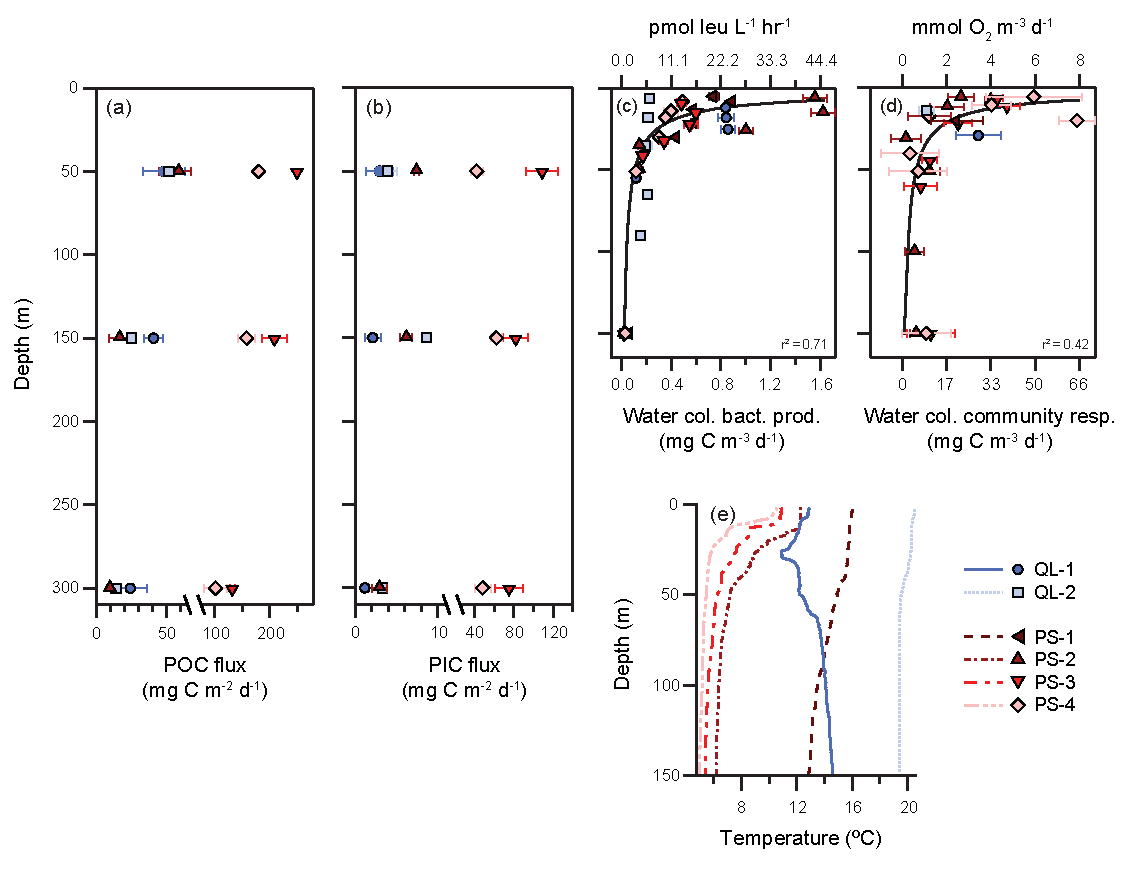
\includegraphics[width=1\textwidth]{Fig_2-3.pdf}
\captionsetup{font={footnotesize}}
\caption[Vertical profiles of sinking carbon fluxes and indicators of community metabolic activity at the six process stations described in the text.]{Vertical profiles of sinking carbon fluxes and indicators of community metabolic activity at the six process stations described in the text. Symbols correspond to those used in \autoref{fig:c2n2} (blue symbols, stations along KN207-1 cruise track; red symbols, KN207-3 stations). Fluxes of sinking (a) POC and (b) PIC were measured using sediment traps at 50, 150, and 300 m. (c) Water column bacterial production. For conversion to units of C in this plot, an isotope dilution (\emph{ID}) of 1 and a conversion factor $\nu _{C:leu}$ of 1.5 kg C (mol leu)\textsuperscript{-1} were employed. A power-law curve (black line, \emph{y} = 10.6 ($\pm$ 0.02) \emph{x} \textsuperscript{-0.69 ($\pm$ 0.01)}; r\textsuperscript{2} = 0.71) was fit by weighted least-squares regression to the data in carbon units. (d) Water column (community) respiration derived from changes in dissolved oxygen concentration in a series of shipboard incubations. We made water-column profiles of community respiration at only three stations (PS-2, PS-3, and PS-4); at the other stations, we made only a single measurement of water column respiration in the euphotic zone. For conversion to units of C, a molar respiratory quotient $\nu _{{\text{C:}}{{\text{O}}_{\text{2}}}}$of 117/170 was used, after Anderson and Sarmiento. A power-law curve (\emph{y} = 169.9 ($\pm$ 3.9) \emph{x} \textsuperscript{-0.74 ($\pm$ 0.01)}; r\textsuperscript{2} = 0.42) was fit as in (c). (e) Also shown are vertical profiles of temperature to 150 m from CTD casts at each of the process stations. Error bars in panels (a), (b), and (c) represent $\pm$ 1$\sigma$ uncertainties derived from replicate (\emph{N} = 3) measurements. Error bars in (d) represent $\pm$ 1$\sigma$ uncertainties derived from the standard error of regression for each set of incubations.}
\label{fig:c2n3}
\end{figure}

Along the westernmost cruise track (KN207-1), a pronounced gradient in surface layer bacterial production was evident in the transition from nutrient replete waters on the continental shelf (those north of the Gulf Stream) to the oligotrophic waters of the Sargasso Sea, at latitudes south of 37$^{\circ}$N. Measured rates of leucine incorporation did not exceed 5 pmol leu L\textsuperscript{-1} h\textsuperscript{-1} anywhere in the water column south of 35.5$^{\circ}$N. These low rates of bacterial production are consistent with the limited inputs of particulate organic substrate that we observed in sediment traps below 50 m at station QL-2, the process station nearest this section of the transect.

We measured the highest rates of bacterial production (\textgreater{}40 pmol leu L\textsuperscript{-1} h\textsuperscript{-1}, equivalent to 1.5 mg C m\textsuperscript{-} d\textsuperscript{-1} assuming $\nu _{C:leu}$ = 1.5 kg C (mol leucine)\textsuperscript{-1} and \emph{ID} = 1) between 52$^{\circ}$N and 54$^{\circ}$N on the eastern KN207-3 cruise transect (\autoref{fig:acn2}b). These sites were associated not with the large particulate carbon fluxes of our subpolar process stations (PS-3 and PS-4), but with the very modest fluxes, we documented at a more southerly station, PS-2. Particulate carbon export at this station was marked by a very pronounced attenuation of flux with depth; 71.7\% and 83.6\% of the POC flux captured at 50 m at this station was attenuated by the time sinking particle material reached the underlying traps at 150 and 300 m, respectively (\autoref{table:c2n3}). These were the sharpest reductions of flux with depth we observed at any location.

The leucine incorporation rates we measured at stations PS-3 and PS-4 were surprisingly low by comparison (\textless{}15 pmol leu L\textsuperscript{-1} h\textsuperscript{-1}; \autoref{fig:acn2}b, to extreme right of plot), despite the development and early senescence (due to active virus infection; K. D. Bidle et al., unpublished data, 2015) of a substantial coccolithophore bloom there during the same period (\autoref{fig:c2n2}b). Evidence from a variety of systems suggests that this is not extraordinary, however. Even in instances when large quantities of particulate carbon are exported to depth, bacterial production may lag primary production and export by days (Ducklow et al., 1993), weeks (Lancelot and Billen, 1984), and, in colder-water ecosystems, months (Azam et al., 1994; Ortega-Retuerta et al., 2014).

Our observations of leucine incorporation (ranging from effectively zero for several stations at 150 m to 51.3 $\pm$ 1.08 pmol leu L\textsuperscript{-1} h\textsuperscript{-1} at station PS-3 at 6 m) agreed with the range of values measured by Hoppe et al\emph{.} (2002) in the North Atlantic surface layer during a transect on the eastern side of the basin (6.52--134 pmol leu L\textsuperscript{-1} h\textsuperscript{-1}, all at 11 m). However, the maximum rates of leucine incorporation we observed were an order of magnitude less than the maximum of 240 pmol leu L\textsuperscript{-1} h\textsuperscript{-1} measured during a previous spring bloom in the western North Atlantic (Li et al., 1993); during that event, rates of 100 pmol leu L\textsuperscript{-1} h\textsuperscript{-1}, still more than double the maximum we observed, were consistently measured at depths \textless{} 20 m. However, at depths \textgreater{} 50 m, the rates measured in that study were nearly at parity with those we report here, suggesting the stimulatory effect of dynamic inputs of sinking carbon may be less significant as depth increases.

\subsection{Respiration Rates}

Profiles of respiration rates in the upper water column (\autoref{fig:c2n3}d) were characterized by a nonlinear decrease in activity with depth that has been broadly documented across marine ecosystems (Reinthaler et al., 2006; Robinson and Williams, 2005). Rates ranged from nearly 8 mmol O\textsubscript{2} m\textsuperscript{-3} d\textsuperscript{-1} in surface waters to those approaching the analytical limit of detection, which was approximately 0.2 mmol O\textsubscript{2} m \textsuperscript{-3} d\textsuperscript{-1}, at depths below 50 m (\autoref{fig:c2n3}d). We found the rate of water column respiration was only weakly predicted by temperature when data for the various stations were aggregated (\emph{p} \textless{} 0.1, \emph{r}\textsuperscript{2} = 0.11; \autoref{fig:c2n4}b); however, a strong (\emph{r}\textsuperscript{2}  \textgreater{} 0.60) positive relationship between \emph{WCR} and temperature was found at some individual stations (PS-2 and PS-3; not shown). By contrast, the decrease with depth we observed in water column respiration was closely paralleled by the trend in bacterial production (\autoref{fig:c2n3}c); the correlation was relatively strong and statistically significant (\emph{p} \textless{} 0.01, \emph{r}\textsuperscript{2} = 0.40; \autoref{fig:c2n4}c).

The decrease in respiration rate with depth was more pronounced at the subpolar site of stations PS-3 and PS-4, where we documented the coccolithophore bloom, than at station PS-2 (\autoref{fig:c2n3}c). The range (0.17--7.9 mmol O\textsubscript{2} m\textsuperscript{-3} d\textsuperscript{-1}) and distribution of the rates we measured (mean $\pm$ standard deviation of all observations, 2.4 $\pm$ 0.8 mmol O\textsubscript{2} m\textsuperscript{-3} d\textsuperscript{-1}) were nearly identical to those of the extensive data set of water column respiration rates compiled by Robinson and Williams (2005). However, when averaged by depth, our rates proved slightly lower than the mean estimates Robinson and Williams reported for the same depth bins (e.g., 3.5 $\pm$ 0.8 versus 4.6 mmol O\textsubscript{2} m\textsuperscript{-3} d\textsuperscript{-1} for data from 0 to 20 m and 0.9 $\pm$ 0.7 versus 1.2 mmol O\textsubscript{2} m\textsuperscript{-3} d\textsuperscript{-1} for 60--200 m). At four stations, we used the traditional two-point Winkler method on samples from the euphotic zone (\emph{N} = 4) to validate our optode sensor spot based bottle measurements (\autoref{table:acn2}). While our incubation measurements generally agreed with the rates we obtained from the Winkler method, the incubations appeared to overestimate the rate of respiration slightly at two stations (or, alternatively, the two-point Winkler method underestimated the true rate; \autoref{fig:acn3} and \autoref{table:acn2}).

\begin{SCfigure}[0.7][!t]
\centering
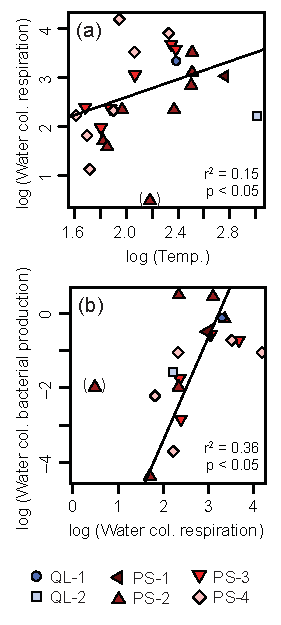
\includegraphics[width=.38\textwidth]{Fig_2-4.pdf}
\captionsetup{font={footnotesize}}
\caption[Relationships between variables transformed by natural logarithm.]{Relationships between variables transformed by natural logarithm. (a) Water column respiration (\emph{WCR}; mg C m\textsuperscript{-3} d\textsuperscript{-1}) versus temperature ($^{\circ}$C). (b) Water column bacterial production (\emph{BP\textsubscript{wc}}; mg C m\textsuperscript{-3} d\textsuperscript{-1}) versus \emph{WCR}. The scatterplots were created using \emph{WCR} and \emph{BP\textsubscript{wc}} data pooled from all stations. In \autoref{fig:c2n4}a, the linear regression \emph{y} = 0.91 ($\pm$0.40) \emph{x} + 0.76 ($\pm$0.88) (black line) was fitted using a weighted ordinary least squares method. In \autoref{fig:c2n4}b, we fitted the linear regression \emph{y} = 2.76 ($\pm$0.42) \emph{x}  - 8.93 ($\pm$1.19) using a type II (major axis---orthogonal distance) method to account for the uncertainties in both variables. We excluded from both regressions the outlier set off with parentheses. Colors and symbols for the various stations correspond to those used in \autoref{fig:c2n2} and \autoref{fig:c2n3}. \emph{WCR} and \emph{BP\textsubscript{wc}} were converted to units of carbon using the same conventions as in \autoref{fig:c2n3}. Uncertainties on regression parameters are $\pm$ 1$\sigma$.}
\label{fig:c2n4}
\end{SCfigure}

The substrate-specific respiration rates we measured on sinking particle material (\emph{k\textsubscript{R}}) spanned an order of magnitude (\autoref{table:c2n2}) and exhibited no clear relationship with depth, water temperature, water column respiration or bacterial production rates, or the magnitude or bulk quality (i.e., rain ratio) of the particulate C flux. The range of values we obtained for \emph{k\textsubscript{R}} (0.007 $\pm$ 0.003 to 0.173 $\pm$ 0.105 d\textsuperscript{-1}) was broader than, yet with a median similar to, the range reported by Sarmiento and Gruber (2006) for \emph{k}\textsubscript{remin}, a model-diagnosed rate constant that encompassed both respiration by particle-attached bacteria and other removal processes (0.02 to 0.1 d\textsuperscript{-1}). Iversen and Ploug (2010) reported a range of values for the carbon-specific respiration rate from 0.08 to 0.20 d\textsuperscript{-1}, based on a compilation of their own measurements and several from the literature. Using an in situ particle incubator in the Sargasso Sea (Bermuda Atlantic Time-series Study site), McDonnell et al. (2015) calculated significantly faster particle ``microbial remineralization rates'' of 0.3 $\pm$ 0.1 to 1.7 $\pm$ 0.4 d\textsuperscript{-1} by normalizing oxygen consumption directly to trap fluxes; these exceeded our sole measurement from the Sargasso (0.084 $\pm$ 0.008, at station QL-2) by an order of magnitude.

The mean value of our \emph{k\textsubscript{R}} measurements for all stations and depths (0.058 $\pm$ 0.011 d\textsuperscript{-1}; \emph{N} = 9 unique observations) agreed with the POC-specific respiration rate of 0.083 d\textsuperscript{-1} calculated by Ploug and Grossart (2000) from roller tank experiments. Working with a natural bacterial assemblage from temperate Pacific waters, Bidle et al. (2002) measured POC-specific remineralization rates on diatom detritus ranging from 0.09 to 0.28 d\textsuperscript{-1}. These rates, which encompassed both particle-attached respiration and processes related to enzymatic solubilization and mechanical disaggregation, were heavily correlated with temperature. Specific remineralization rates of the biogenic silica in the same detritus ranged from 1.1 to 49\% of the corresponding POC-specific rate.

\section{Model Results and Discussion}

\subsection{Sensitivity Analyses}

We compared our model results --- POC flux predictions based on ranges of values for \emph{k\textsubscript{S}}\textsubscript{,\emph{D},\emph{Z}} and \emph{W\textsubscript{avg}} --- to observations of POC flux at two depth intervals for each of five process stations (\autoref{fig:c2n5}). Relatively narrow confidence regions in 6 of our 10 analyses allowed us to place both upper and lower constraints on the agreement between our predictions and observations (\autoref{fig:c2n5}; confidence regions are shaded and enclosed within dashed lines). However, in four cases (both depth intervals at station QL-1, the 150-300 m interval at PS-2, and the 50-150 m interval at PS-4), large uncertainties in either the observed fluxes or in our inputs of \emph{k\textsubscript{R}} prevented us from assigning significance to the model-observed deviations, except at very slow sinking speeds. The six analyses that produced narrower confidence regions offer several insights into the partitioning between processes that drive particle flux attenuation (\autoref{sssec:Partitioning of Sinking POC Flux Attenuation Between Direct Bacterial Respiration and Other Degradation Processes}, below).

\subsubsection{Minimum Constraints on Average Particle Sinking Velocity}
\label{sssec:Minimum Constraints on Average Particle Sinking Velocity}

We diagnosed a statistically significant minimum constraint on \emph{W\textsubscript{avg}} at all depth intervals to which we applied a sensitivity analysis (\autoref{table:c2n3}). At slow average sinking velocities (\autoref{fig:c2n5}, to extreme left in each plot), we obtained low uncertainties from the model over the entire range of values we considered for \emph{k\textsubscript{S}}\textsubscript{,\emph{D},\emph{Z}}; this allowed us to exclude completely from the solution space values of \emph{W\textsubscript{avg}} that fell below a certain threshold. The minimum bound on \emph{W\textsubscript{avg}} we obtained in this manner ranged from 2.8 m d\textsuperscript{-1} to 16.8 m d\textsuperscript{-1} (mean $\pm$ standard deviation, 9.3 $\pm$ 4.3 m d\textsuperscript{-1}). There was no statistically significant difference between the average minimum bounds for the two depth intervals.

While the form of our analysis did not allow us to estimate a central, best fit value for \emph{W\textsubscript{avg}} at each station, the minimum constraints we obtained are consistent with previous observations of the average particle sinking velocity at a diversity of sites in the mesopelagic North Atlantic Ocean (\autoref{table:acn1}). Although sinking velocities \textless{} 1 m d\textsuperscript{-1} have been reported for cell material from individual cultures of certain phytoplankton species (Bach et al., 2012) and for certain lithogenic particles of Aeolian origin (Ohnemus and Lam, 2014), a median \emph{W\textsubscript{avg}} of 50 m d\textsuperscript{-1} (interquartile range, 11.5--100 m d\textsuperscript{-1}; mean, 63.8 m d\textsuperscript{-1}) emerged from a data set of observations we assembled from the literature for the temperate North Atlantic Ocean at depths \textless{} 1000 m (\autoref{table:acn1} and \autoref{fig:c2n5}). Average particle sinking velocities well in excess of 500 m d\textsuperscript{-1} have been reported in other ocean basins and at depths \textgreater{} 1500 m (Berelson, 2002; McDonnell et al., 2015; Stemmann et al., 2004a). In instances where a bimodal distribution of particle sinking velocities has been observed in the North Atlantic, a slow-sinking particle size fraction can be complemented by a fast-sinking fraction with an average sinking velocity of nearly 200 m d\textsuperscript{-1} (Riley et al., 2012). Of course, regardless of the system, \emph{W\textsubscript{avg}} is a function of a heterogeneous distribution of individual sinking speeds attached to different particle size classes (McDonnell and Buesseler, 2010; Villa-Alfageme et al., 2014). Despite the lack of correlation in this case between \emph{k\textsubscript{R}} and the ratio of POC:PIC in the sinking flux (i.e., the rain ratio; \autoref{table:c2n2}), we did identify a weak (\emph{r}\textsuperscript{2} = 0.19) and barely significant (\emph{p} = 0.1) negative correlation between our minimum estimates of \emph{W\textsubscript{avg}} and the rain ratio. This result follows the finding of a recent, culture-based laboratory study suggesting concentrations of biogenic PIC can enhance bulk particle sinking speed even when little effect is seen on the substrate-specific respiration rate (Iversen and Ploug, 2010). Conversely, Lam et al. (2011) have suggested that the high mesopelagic transfer efficiencies associated with CaCO\textsubscript{3}-rich organic matter may be less a function of faster sinking velocity than the result of an inherent complexity in such organic matter that renders it less amenable to direct respiration.

\subsubsection{Partitioning of Sinking POC Flux Attenuation Between Direct Bacterial Respiration and Other Degradation Processes}
\label{sssec:Partitioning of Sinking POC Flux Attenuation Between Direct Bacterial Respiration and Other Degradation Processes}

Several sets of values of \emph{W\textsubscript{avg}} and \emph{k\textsubscript{S}}\textsubscript{,\emph{D},\emph{Z}} minimized the deviation between the modeled and observed fluxes at each station; these are the pairs of values that fall along the ``0'' isoline in each of the plots in \autoref{fig:c2n5}. To constrain this set of possible solutions and obtain best fit estimates for \emph{k\textsubscript{S}}\textsubscript{,\emph{D},\emph{Z}} in each case, we sought to limit our assessment of \emph{k\textsubscript{S}}\textsubscript{,\emph{D},\emph{Z}} to those values of \emph{W\textsubscript{avg}} that were most plausible for the North Atlantic. We chose 50 m d\textsuperscript{-1}, the median value of the data set we assembled from the literature (\autoref{fig:c2n5} and \autoref{table:acn1}; \emph{N} = 72 individual observations of \emph{W\textsubscript{avg}}), as the average sinking velocity for which we report a best fit value for \emph{k\textsubscript{S}}\textsubscript{,\emph{D},\emph{Z}} in each case. Using this criterion, we obtained estimates of \emph{k\textsubscript{S}}\textsubscript{,\emph{D},\emph{Z}} and accompanying uncertainties of $0.015_{ - 0.02}^{ + 0.15}$ to $0.57_{ - 0.30}^{ + 0.43}$ d\textsuperscript{-1} (\autoref{table:c2n3}; mean $\pm$ standard deviation, 0.16 $\pm$ 0.17 d\textsuperscript{-1}). These estimates are the values in \autoref{fig:c2n5} (denoted with + symbol) where the vertical line corresponding to 50 m d\textsuperscript{-1} intersects the $\Delta$(model-observed) ``0'' isoline and the boundaries of the confidence region. To estimate the relative contribution to sinking POC flux attenuation of the processes represented in \emph{k\textsubscript{S}}\textsubscript{,\emph{D},\emph{Z}} compared with respiration of particle material by attached bacteria, we calculated the ratio of the two rate constants, \emph{k\textsubscript{S}}\textsubscript{,\emph{D},\emph{Z}} : \emph{k\textsubscript{R}}. This ratio ranged from 0.3 over the 50--150 m interval at station PS-4 to 11.2 over the same interval at station PS-2. The mean ratio of the two rate constants was 3.4, although the distribution was highly scattered (standard deviation = 4.0).

\begin{figure}[!p]
\includegraphics[width=1\textwidth]{Fig_2-5.pdf}
\end{figure}

In the following sense, we believe these values represent a conservative estimate of the predominance of other degradation processes over the respiration of sinking particles by attached bacteria. Our diagnostic approach depends on the value we assume for \emph{W\textsubscript{avg}}; we applied the median value of 50 m d\textsuperscript{-1} from our survey of the literature. If the true average sinking velocity at any station were faster than 50 m d\textsuperscript{-1}, we would therefore have underestimated \emph{k\textsubscript{S}}\textsubscript{,\emph{D},\emph{Z}} (and, by extension, the ratio of \emph{k\textsubscript{S}}\textsubscript{,\emph{D},\emph{Z}} : \emph{k\textsubscript{R}}). We suspect the average sinking velocity at our sites could well have been faster, particularly at the stations where primary production was dominated by coccolithophores (PS-3 and PS-4; \autoref{table:c2n2}). The one study in our literature survey to report average sinking velocities for particles specifically associated with a coccolithophore bloom estimated a \emph{W\textsubscript{avg}} of 141 $\pm$ 11 m d\textsuperscript{-1}, nearly 3 times that of the 50 m d\textsuperscript{-1} we selected (Knappertsbusch and Brummer, 1995). During a summer coccolithophore bloom in the equatorial Atlantic, Fischer and Karakas (2009) measured average particle sinking velocities of almost 570 m d\textsuperscript{-1}. Given the shapes of the curves that result from the exponential decay model, a small upward revision in \emph{W\textsubscript{avg}} from a starting value of 50 m d\textsuperscript{-1} would have little impact on our diagnosis. For example, in all instances except for the 150--300 m depth interval at station QL-1, an increase in \emph{W\textsubscript{avg}} from 50 to 75 m d\textsuperscript{-1} would produce only a modest change in the value of \emph{k\textsubscript{S}}\textsubscript{,\emph{D},\emph{Z}}, since this is region where the ``0'' isoline curve begins to approach an asymptote (\autoref{fig:c2n5}).
\begin{figure} [!t]
\captionsetup{font={footnotesize}}
\captionof{figure}[Sensitivity analyses of the particle flux attenuation model by station and depth interval.]{(preceding page). Sensitivity analyses of the particle flux attenuation model by station and depth interval. We evaluated variation in two parameters, the average particle sinking velocity (\emph{W\textsubscript{avg}}, from 1 to 200 m d\textsuperscript{-1}; \emph{x}-axis) and \emph{k\textsubscript{S}}\textsubscript{,\emph{D},\emph{Z}}, an activity constant that captures losses of sinking POC due to processes other than direct respiration by particle-attached bacteria (\emph{y}-axis; from 10\textsuperscript{-5} to 1 d\textsuperscript{-1}; \autoref{fig:c2n1}). Colorbar ramp and labeled contour lines indicate, for a given pair of values of \emph{W\textsubscript{avg}} and \emph{k\textsubscript{S}}\textsubscript{,\emph{D},\emph{Z}}, deviation of the model result from the observed POC flux at that station, in units of mg C m\textsuperscript{-2} d\textsuperscript{-1}. Left panels: Results for 50-150 m. Right panels: Results for 150-300 m. The secondary \emph{y}-axis (ratio of \emph{k\textsubscript{S}}\textsubscript{,\emph{D},\emph{Z}} to \emph{k\textsubscript{R}}, the measured substrate-specific rate of respiration on sinking particles) shows the relative contribution to particle flux attenuation at each station by respiration compared to the other processes that degrade sinking particles. The shaded area in each plot encompassed by the dashed line is a 1$\sigma$ ({\raise.17ex\hbox{$\scriptstyle\sim$}} 68\%) confidence region derived from uncertainties in the model solutions and observed flux at that station. Model-observed deviations outside this region are statistically significant. Also shown above each set of plots is an identical histogram of relevant observations (\emph{N} = 72) of average sinking velocities in the North Atlantic; the assembly of these data is described in \autoref{sssec:Minimum Constraints on Average Particle Sinking Velocity} of the text. The median (50 m d\textsuperscript{-1}; band at center of box plot) and IQR (11.5-100 m d\textsuperscript{-1}) are shown in the accompanying boxplot. Whiskers extend to 1.5 IQR. The sole reported value \textgreater{} 200 m d\textsuperscript{-1} (250 m d\textsuperscript{-1}) was excluded as an outlier.}
\label{fig:c2n5}
\end{figure}

We take the results of our analysis to indicate that, at minimum, the majority of sinking particle material attenuated between 50 and 300 m did not meet its ultimate fate through direct respiration by attached bacteria. Instead, the results suggest a significant fraction of the sinking particulate flux was transferred to the water column as suspended particulate or dissolved organic matter, at least some of it providing a metabolic subsidy to the free-living bacterial community. Because some of the sinking POC flux might have been directly respired by associated zooplankton, we cannot be certain \emph{k\textsubscript{S}}\textsubscript{,\emph{D},\emph{Z}} exclusively represents the transfer of mass to the water column. However, while carbon demand incurred by zooplankton is an important sink in some marine systems such as the central equatorial Pacific (Landry et al., 1997), subarctic Pacific (Steinberg et al., 2008b), and at station ALOHA (Steinberg et al., 2008a), the results of the North Atlantic Bloom Experiment suggest zooplankton are much less significant players in midlatitude or subpolar North Atlantic systems during bloom conditions (Dam et al., 1993). In this case, we hypothesize that the major role played by zooplankton was instead that of mechanical disaggregator, complementing enzymatic solubilization by particle-attached bacteria in transferring carbon to the dissolved and suspended particulate phases.

The hypothesized transfer of organic matter from the sinking particulate to suspended or dissolved phases is supported by theoretical and laboratory studies (Alldredge, 2000; Bendtsen et al., 2002; Grossart and Simon, 1998; Ki\o{}rboe and Jackson, 2001), evidence from other field-based research (Giering et al., 2014; Smith et al., 1992; Taylor and Karl, 1991), and, at stations PS-2, PS-3, and PS-4, by very high rates of depth-integrated water column respiration from 50 to 150 m (465.2 $\pm$ 182.1 to 887.09 $\pm$ 456.2 mg C m\textsuperscript{-2} d\textsuperscript{-1}; mean $\pm$ standard deviation, 729.3 $\pm$ 266.0 mg C m\textsuperscript{-2} d\textsuperscript{-1}; \autoref{table:c2n3}). Intriguingly, we could find no direct statistical correlations between our estimates of the \emph{k\textsubscript{S}}\textsubscript{,\emph{D},\emph{Z}} : \emph{k\textsubscript{R}} ratio (or \emph{k\textsubscript{S}}\textsubscript{,\emph{D},\emph{Z}} itself) and any of the other parameters we measured. In the cases of \emph{BP\textsubscript{wc}}, \emph{WCR}\textsubscript{int}, and \emph{BGE}\textsubscript{pa} specifically, we did not have enough observations of the parameters to make a statistical assessment (\autoref{table:c2n2} and \autoref{table:c2n3}).

While our analysis did not allow us to identify the specific mechanisms by which this mass transfer might have occurred, our finding is general in nature and therefore accommodates all of the degradation processes we considered in our initial conceptualization of particle flux attenuation (\autoref{fig:c2n1}). In balancing a carbon budget for a site roughly 1000 km southeast of our PS-2 station, Giering et al. (2014) hypothesized that mechanical fragmentation by zooplankton had diverted nearly a third of fast-sinking particles to the dissolved and suspended phases, where the carbon they contained was then respired by bacteria. Mayor et al. (2014) described this apparent dynamic as a manifestation of Fenchel's (1970) ``microbial gardening'' hypothesis. Because so much of the sinking POC appeared to meet its ultimate fate in the water column, Giering et al. chose to construct their budget around indirect estimates of the depth-integrated water column respiration rate, which they contended best captured the total metabolic sink imposed by the microbial community.

Drawing on observations from the North Pacific, Taylor and Karl (1991) concluded that the inefficient metabolism of sinking particles by attached microbiota was likely reflected in a large transfer of organic matter to the suspended and dissolved phases. This is the roughly the same hypothesis advanced by Smith et al. (1992), who based their speculation on the very intense ectohydrolytic enzyme activity and low direct carbon demand they measured on sinking particle material. Other authors have also used observations and manipulations of particle material to argue for the importance of this mechanism in carbon transfer (Alldredge, 2000; Grossart and Simon, 1998). Ki\o{}rboe and Jackson (2001) later used results from a series of models to estimate that the dissolved organic matter left behind in the wake of a sinking particle could provide a very significant subsidy to the surrounding water column; Bendtsen et al\emph{.} (2002) concluded based on a larger-scale modeling analysis that solubilization of particle material was a significant source of DOC in the deep ocean.

In invoking this mechanism as a possible explanation for their findings, Taylor and Karl (1991) noted that any form of disaggregation or solubilization necessarily introduces a time lag between components of the ecosystem metabolic engine. The sinking organic matter not directly respired by attached bacteria --- as we hypothesize, a majority, or at least a significant fraction, of the sinking POC at our sites --- will not necessarily become immediate metabolic substrate for microbes in the water column. Consistent with observations from a variety of marine systems (see our brief discussion in \autoref{ssec:Bacterial Production}, above), this DOM or suspended POM may linger for weeks, months, or years before it is respired; some fraction will become part of the recalcitrant dissolved organic matter pool. Solubilization of sinking particles and the fraction of solubilized material that is directly respired by attached bacteria are therefore directly intertwined, even when the majority of the solubilized material is instead transferred to the water column.

Ki\o{}rboe et al. (2002) have further suggested that some loss of sinking particle mass can be explained by the shedding of live bacterial cells, which abandon the particle for the water column. Given the low bacterial growth efficiencies we observed on both sinking particles and in the water column (\autoref{table:c2n2}), we suspect this mechanism of particle loss was probably not significant in the present study.

\subsubsection{Enigmatically Low Efficiencies of Bacterial Growth}
\label{sssec:Enigmatically Low Efficiencies of Bacterial Growth}

We used our observations of water column bacterial production and respiration to calculate the water column \emph{BGE} (\emph{BGE\textsubscript{wc}}) at stations PS-2, PS-3, and PS-4 (\autoref{table:c2n2}). At stations QL-1 and QL-2, complementary measurements allowed us to calculate analogous values on sinking particles (\autoref{table:c2n2}). Bacterial growth in both carbon reservoirs proved generally inefficient, but our estimates of \emph{BGE} in the water column at depths $\geq$ 50 m were extraordinary low (0.001 $\pm$ 0.001 to 0.014 $\pm$ 0.012; mean $\pm$ standard deviation, 0.006 $\pm$ 0.002). Estimates of \emph{BGE\textsubscript{wc}} as low as 0.001 have been reported for depths below the mixed layer (90 m) in the highly oligotrophic Mediterranean Sea (Lem\'{e}e et al., 2002), and Reinthaler et al. (2006) reported growth efficiencies of just 0.006-0.016 in deep waters (\textgreater{}1200 m) of the North Atlantic. By contrast, \emph{BGE}s of 0.09 to 0.38 were estimated for the Ross Sea surface layer during a bloom of \emph{Phaeocystis} (Carlson et al., 1999). However, in the latter case, one might expect that the substrate available to the bacterial community was considerably more amenable to metabolism than either the sinking particles or the dissolved and suspended organic matter derived from them.

We believe for several reasons that our estimates are minimum bounds on water column \emph{BGE}. Since we used unfiltered water samples in our incubations, constituents of the water column microbial community other than prokaryotes (nanozooplankton, protists, and even some phytoplankton) could have contributed to the observed consumption of oxygen if they were present. Although we controlled for the presence of macrozooplankton by visual inspection, Ki\o{}rboe (2001) notes that it is virtually impossible to distinguish between bacteria and other smaller microorganisms such as protozoans. If we assume conservatively that these other organisms contributed as much to respiration as did bacteria, our mean estimate of \emph{BGE\textsubscript{wc}} for depths $\geq$ 50 m would roughly double to 0.01 $\pm$ 0.004. Additionally, flaws inherent in the \textsuperscript{3}H-leucine incorporation method, or in our choice of values for \emph{ID} or $\nu _{C:leu}$, could have caused us to significantly underestimate rates of bacterial production. The large uncertainties we introduced into our estimates of depth-integrated BP when we considered variation in both of the conversion factors (uncertainties represented 60\%, on average, of the accompanying estimate; \autoref{table:c2n3}) demonstrate how a broad range of possible values can be extrapolated from a single set of leucine incorporation measurements. For example, if we also discarded our conservative assumption for \emph{ID} and instead adopted a value of 2 --- assuming bacteria incorporated as much radiolabeled leucine into protein as endogenous leucine (Kirchman, 2001) --- our mean estimate of \emph{BGE\textsubscript{wc}} could be as high as 0.04.

However, the fact remains that when considered independently, our observations of both bacterial production and water column respiration are highly consistent with the large sets of values previously reported for the North Atlantic for both parameters. Critically, even a \emph{BGE} of 0.04 --- the highest possible value we could accept obtaining from our observations under the hypothetical scenario above --- would still be considerably lower than the 0.15 applied by Steinberg et al. (2008b) or the median value of 0.08 Giering et al. (2014) obtained from an assembled data set; those studies represent two of the most prominent attempts to balance carbon budgets in the mesopelagic ocean on an ecosystem scale.

\subsubsection{Possible Imbalances in the North Atlantic Carbon Budget}

If, as Giering et al. (2014) and others have contended, depth-integrated water column bacterial respiration is the primary carbon sink in a given marine ecosystem, our data suggest a very substantial imbalance existed in the carbon budgets of our study sites, at least over the spatial and temporal scales we considered. At the three stations (PS-2, PS-3, and PS-4) for which we had concurrent measurements of the relevant parameters, the metabolic sink imposed by \emph{WCR\textsubscript{int}} over the 50 to 150 m depth interval surpassed observed attenuation in sinking POC flux over the same interval by an average of more than 26 times (\autoref{table:c2n3}). There are very few sediment trap- or \textsuperscript{234}Th-derived observations of POC fluxes in the literature that would have supplied a quantity of carbon sufficient to satisfy the respiratory demand we measured; for example, the 940.4 mg C m\textsuperscript{-2} d\textsuperscript{-1} observed by Le Moigne et al., 2015) in the Atlantic sector of the Arctic Ocean is remarkably high. No observations previously reported for the sub-Arctic North Atlantic would have satisfied the metabolic demand imposed by our observations of \emph{WCR\textsubscript{int}}.

Depth-integrated water column BP comprised such a small fraction of \emph{WCR\textsubscript{int}} at each site (\autoref{table:c2n3}) that the substantial uncertainties we introduced into our calculations of \emph{BP\textsubscript{int}} by incorporating variation in \emph{ID} and $\nu _{C:leu}$ were of relatively little consequence. Our bootstrap analysis indicated that variation in the two conversion factors accounted for more than 90\% of the uncertainties in our estimates of \emph{BP\textsubscript{int}}. We acknowledge here that, if instead of measuring respiration directly, we had extrapolated estimates of \emph{WCR\textsubscript{int}} from these measurements of BP (as did Giering et al. (2014)), these uncertainties would have become extremely consequential. Further, if some systematic bias in our incubation technique caused us to overestimate individual rates of \emph{WCR} by even a small amount, the offset would have produced a large positive deviation upon vertical integration.

Even if our calculations of \emph{WCR\textsubscript{int}} represented a twofold overestimate of the metabolic demand imposed by bacteria (based on the same logic we invoke in our discussion of \emph{BGE}; \autoref{sssec:Enigmatically Low Efficiencies of Bacterial Growth}, above), the carbon budgets at these three sites could only be closed by large lateral or vertical inputs of DOC, or by some other unknown source of reducing power. Zooplankton respiration in the water column --- a sink we did not measure or estimate --- would supply additional oxidizing power in excess of that already captured in \emph{WCR\textsubscript{int}}, creating a demand for even more reduced carbon. Giering et al. estimated that inputs of DOC supplied 17\% of the carbon needed to balance the metabolic budget they created in their study; similar values have been reported elsewhere in the North Atlantic (Carlson et al., 2010), though evidence suggests the fraction of export supplied by DOC could be even higher ($\sim 29$\%) in oligotrophic waters of the Sargasso Sea (Carlson et al., 1994). Inputs of DOC on the order of that observed in those studies could narrow the metabolic disparity at our sites significantly, but would be insufficient to close the gap completely.

Alternatively, our bottle-based measurements of \emph{WCR\textsubscript{int}} could be significant overestimates that reflect a methodological bias. Bottle-based methods for measuring respiration or other metabolic processes in marine microorganisms are prone to error from (1) contamination and disruption introduced through the process of obtaining seawater samples and preparing them for incubation, including the effects of depressurization when samples are collected from depth (Tamburini et al., 2013); (2) unrepresentative incubation conditions that do not faithfully reproduce the variations in temperature and light inherent in natural systems; and (3) so-called ``bottle effects'' associated with low-volume incubations which may limit nutrient availability (Furnas, 2002) or induce unnatural changes in community structure (Calvo-D\'{i}az et al., 2011; Venrick et al., 1977).

Our data thus suggest balance in the North Atlantic carbon budget remains elusive, likely due to some combination methodological limitations, a failure to account for some critical additional flux, or a failure to consider adequately the time scales of those sources and sinks we did measure. Despite a handful of successful attempts at balancing marine carbon budgets on ecosystem (Giering et al., 2014) and basin scales (Williams et al., 2013), we arrive by different methods at the same vexing problem that confronted Steinberg et al. (2008b): A system that apparently out of metabolic balance. This imbalance notwithstanding, the strong oxidizing power in the depth-integrated respiration rates we observed still supports our hypothesis for a significant transfer of sinking particulate carbon to the water column. Insofar as this mass transfer is concerned, the apparent metabolic imbalance simply indicates that carbon evolved from sinking particle material is alone insufficient to supply the necessary reducing power.

\section{Conclusion}

The relative strength --- and apparent predominance, at the majority of sites in this study --- of the other biological and mechanical processes that compete with direct respiration to degrade sinking particles suggest the mesopelagic ocean is characterized by a distinct remineralization regime in which hydrolysis and respiration are significantly decoupled. Sinking organic matter transferred to the dissolved or suspended particulate phases through enzymatic solubilization or mechanical disaggregation provides a considerable metabolic subsidy to the water column microbial community. Yet evidence from other studies suggests the respiration of this organic matter may lag its transfer from the sinking particulate phase by weeks, months, or years. This temporal disconnect makes it difficult to diagnose the exact mechanisms of organic matter transfer from the sinking particulate phase and hinders accurate appraisal of the flux's magnitude.

The large disparity we documented between rates of depth-integrated water column respiration and attenuation of sinking POC is further evidence that our methods of characterizing microbial metabolisms remain inadequate, or that our knowledge of the various reservoirs and fluxes that define the marine carbon cycle remains incomplete. The very low bacterial growth efficiencies we observed in this study are further evidence for both of these deficiencies. The variation in \emph{BGE} we observed both in the water column and on the sinking particles suggests that the lability of particulate organic matter can be altered as it is exported to depth.

One way to diagnose apparent carbon budget discrepancies is by pairing incubation-based techniques such as those we employed with concurrent measurements based on in situ geochemical tracer techniques that integrate more broadly over both time and space (e.g., Quay et al., 2010). For example, at steady state, a respiratory sink of the magnitude we measured would have required some complementary source of dissolved oxygen; otherwise, we would have expected to observe at some timescale a significant decrease in dissolved oxygen inventory. Concurrent measurements of dissolved oxygen anomalies (e.g., Najjar and Keeling, 1997) or apparent oxygen utilization (e.g., Stanley et al., 2012) might have allowed us to determine whether this metabolic demand was in fact balanced over seasonal or annual timescales by other processes.

Despite a handful of recent studies that have successfully balanced carbon budgets for sectors of the North Atlantic, we find strong justification here for the further development of new analytical methods and new hypotheses about how the carbon cycle functions. At the same time, the rates of water column respiration that drove this apparent imbalance provide support for our hypothesis that degradation processes other than direct respiration can dominate particle flux attenuation. Investigators seeking to accurately characterize the marine carbon cycle with new mechanistic models of production and export should endeavor to incorporate these other processes to an extent equal to that of respiration.

\section{Acknowledgments}

We thank the captains and crew of the R/V \emph{Knorr}, as well as Jamey Fulton, Anton Zafereo, David Sims, Filipa Carvalho, Helen Fredricks, Dan McCorkle, Valier Galy, Krista Longnecker, Suni Shah, Dave Glover, Carl Johnson, Olivia De Meo, Steve Manganini, Phoebe Lam, Joe Salisbury, and Maria Kavanaugh. Elizabeth Kujawinski provided thoughtful comments on an earlier version of the manuscript. We are lastly grateful to Hugh Ducklow and to two anonymous reviewers, whose criticism improved the manuscript dramatically. J.R.C. acknowledges support from a U.S. Environmental Protection Agency (EPA) STAR Graduate Fellowship (Fellowship Assistance agreement FP-91744301-0). The contents of this research have not been formally reviewed by EPA. The views expressed in this manuscript are solely those of the authors, and EPA does not endorse any products or commercial services mentioned therein. K.D.B. acknowledges support from the National Science Foundation (NSF OCE-1061883) and the Gordon and Betty Moore Foundation (3301 and 3789). S.C.D. acknowledges support from the National Science Foundation through the Center for Microbial Oceanography: Research and Education (C-MORE) (NSF EF-0424599). B.A.S.V.M. acknowledges support from the National Science Foundation (NSF OCE-1155438, OCE-1059884, and OCE-1031143), the Gordon and Betty Moore Foundation, and the Woods Hole Oceanographic Institution through a Cecil and Ida Green Foundation Innovative Technology Award and an Interdisciplinary Science Award.

\section{Availability of Data and Code }

Curated oceanographic data can be found on the BCO-DMO web site at \url{http://www.bco-dmo.org/deployment/58787} (KN207-1) and \url{http://www.bco-dmo.org/project/2136} (KN207-3). Additional data and all code used to produce the figures and analysis in this chapter are contained in GitHub repositories at \texttt{\href{https://github.com/jamesrco/MultipleFatesofParticles}{https://github.com/jamesrco/MultipleF\\atesofParticles}} and (for analysis of bacterial production data) \url{https://github.com/jamesrco/3H_Leu_BactProd}

\clearpage
\begin{singlespace}
\section*{References}
\addtocounter{section}{1}
{\setlength{\parindent}{0pt}
Alldredge, A. L. (2000), Interstitial dissolved organic carbon (DOC) concentrations within sinking marine aggregates and their potential contribution to carbon flux, \emph{Limnology \& Oceanography}, 45(6), 1245-1253.

{\setlength{\parskip}{10pt}

Alldredge, A. L., T. C. Granata, C. C. Gotschalk, and T. D. Dickey (1990), The physical strength of marine snow and its implications for particle disaggregation in the ocean, \emph{Limnology \& Oceanography}, 35(7), 1415-1428.

Alonso-Saez, L., et al. (2008), Factors controlling the year-round variability in carbon flux through bacteria in a coastal marine system, \emph{Ecosystems}, 11(3), 397-409, doi:\href{http://dx.doi.org/10.1007/S10021-008-9129-0}{10.1007/S10021-008-9129-0}.

Anderson, L. A., and J. L. Sarmiento (1994), Redfield ratios of remineralization determined by nutrient data-analysis, \emph{Global Biogeochemical Cycles}, 8(1), 65-80, doi:\href{http://dx.doi.org/10.1029/93GB03318}{10.1029/93GB03318}.

Anderson, T. R., and K. W. Tang (2010), Carbon cycling and POC turnover in the mesopelagic zone of the ocean: Insights from a simple model, \emph{Deep Sea Research Part II: Topical Studies in Oceanography}, 57(16), 1581-1592, doi:\href{http://dx.doi.org/10.1016/j.dsr2.2010.02.024}{10.1016/j.dsr2.2010.02.024}.

Aranguren-Gassis, M., P. Serret, E. Fern\'{a}ndez, J. L. Herrera, J. F. Dom\'{i}nguez, V. P\'{e}rez, and J. Escanez (2012), Balanced plankton net community metabolism in the oligotrophic North Atlantic subtropical gyre from Lagrangian observations, \emph{Deep Sea Research Part I: Oceanographic Research Papers}, 68, 116-122, doi:\href{http://dx.doi.org/10.1016/j.dsr.2012.06.004}{10.1016/j.dsr.2012.06.004}.

Azam, F. (1998), Microbial control of oceanic carbon flux: The plot thickens, \emph{Science}, 280(5364), 694-696, doi:\href{http://dx.doi.org/10.1126/science.280.5364.694}{10.1126/science.280.5364.694}.

Azam, F., and F. Malfatti (2007), Microbial structuring of marine ecosystems, \emph{Nature Reviews Microbiology}, 5(10), 782-791.

Azam, F., D. C. Smith, G. F. Steward, and \AA{}. Hagstr\"{o}m (1994), Bacteria-organic matter coupling and its significance for oceanic carbon cycling, \emph{Microbial Ecology}, 28(2), 167-179, doi:\href{http://dx.doi.org/10.1007/BF00166806}{10.1007/BF00166806}.

Bach, L. T., U. Riebesell, S. Sett, S. Febiri, P. Rzepka, and K. G. Schulz (2012), An approach for particle sinking velocity measurements in the 3-400 $\mu$m size range and considerations on the effect of temperature on sinking rates, \emph{Marine Biology}, 159(8), 1853-1864, doi:\href{http://dx.doi.org/10.1007/S00227-012-1945-2}{10.1007/S00227-012-1945-2}.

Bendtsen, J., C. Lundsgaard, M. Middelboe, and D. Archer (2002), Influence of bacterial uptake on deep-ocean dissolved organic carbon, \emph{Global Biogeochemical Cycles}, 16(4), 1127, doi:\href{http://dx.doi.org/10.1029/2002GB001947}{10.1029/2002GB001947}.

Berelson, W. M. (2002), Particle settling rates increase with depth in the ocean, \emph{Deep Sea Research Part II: Topical Studies in Oceanography}, 49(1-3), 237-251.

Bidle, K. D., M. Manganelli, and F. Azam (2002), Regulation of oceanic silicon and carbon preservation by temperature control on bacteria, \emph{Science}, 298(5600), 1980-1984, doi:\href{http://dx.doi.org/10.1126/science.1076076}{10.1126/\\science.1076076}.

Boyd, P. W., and T. W. Trull (2007), Understanding the export of biogenic particles in oceanic waters: Is there consensus?, \emph{Progress in Oceanography}, 72(4), 276-312, doi:\href{http://dx.doi.org/10.1016/J.Pocean.2006.10.007}{10.1016/J\\.Pocean.2006.10.007}.

Buesseler, K. O., and P. W. Boyd (2009), Shedding light on processes that control particle export and flux attenuation in the twilight zone of the open ocean, \emph{Limnology \& Oceanography}, 54(4), 1210-1232, doi:\href{http://dx.doi.org/10.4319/lo.2009.54.4.1210}{10.4319/lo.2009.54.4.1210}.

Buesseler, K. O., et al. (2007a), An assessment of the use of sediment traps for estimating upper ocean particle fluxes, \emph{Journal of Marine Research}, 65(3), 345-416.

Buesseler, K. O., et al. (2007b), Revisiting carbon flux through the ocean's twilight zone, \emph{Science}, 316(5824), 567-570, doi:\href{http://dx.doi.org/10.1126/science.1137959}{10.1126/science.1137959}.

Burd, A. B. (2013), Modeling particle aggregation using size class and size spectrum approaches, \emph{Journal of Geophysical Research: Oceans}, 118, 3431-3443, doi:\href{http://dx.doi.org/10.1002/Jgrc.20255}{10.1002/Jgrc.20255}.

Burd, A. B., et al. (2010), Assessing the apparent imbalance between geochemical and biochemical indicators of meso- and bathypelagic biological activity: What the @\$\#! is wrong with present calculations of carbon budgets?, \emph{Deep Sea Research Part II: Topical Studies in Oceanography}, 57(16), 1557-1571, doi:\href{http://dx.doi.org/10.1016/J.Dsr2.2010.02.022}{10.1016/J.Dsr2.2010.02.022}.

Calvo-D\'{i}az, A., L. D\'{i}az-P\'{e}rez, L. \'{a}. Su\'{a}rez, X. A. G. Mor\'{a}n, E. Teira, and E. Mara\~{n}\'{o}n (2011), Decrease in the autotrophic-to-heterotrophic biomass ratio of picoplankton in oligotrophic marine waters due to bottle enclosure, \emph{Applied and Environmental Microbiology}, 77(16), 5739-5746, doi:\href{http://dx.doi.org/10.1128/aem.00066-11}{10.1128/aem.00066-11}.

Carlson, C. A., H. W. Ducklow, and A. F. Michaels (1994), Annual flux of dissolved organic carbon from the euphotic zone in the northwestern Sargasso Sea, \emph{Nature}, 371(6496), 405-408.

Carlson, C. A., N. R. Bates, H. W. Ducklow, and D. A. Hansell (1999), Estimation of bacterial respiration and growth efficiency in the Ross Sea, Antarctica, \emph{Aquatic Microbial Ecology}, 19(3), 229-244, doi:\href{http://dx.doi.org/10.3354/ame019229}{10.3354/ame019229}.

Carlson, C. A., D. A. Hansell, N. B. Nelson, D. A. Siegel, W. M. Smethie, S. Khatiwala, M. M. Meyers, and E. Halewood (2010), Dissolved organic carbon export and subsequent remineralization in the mesopelagic and bathypelagic realms of the North Atlantic basin, \emph{Deep Sea Research Part II: Topical Studies in Oceanography}, 57(16), 1433-1445, doi:\href{http://dx.doi.org/10.1016/j.dsr2.2010.02.013}{10.1016/j.dsr2.2010.02.013}.

Chin-Leo, G., and D. L. Kirchman (1988), Estimating bacterial production in marine waters from the simultaneous incorporation of thymidine and leucine, \emph{Applied and Environmental Microbiology}, 54(8), 1934-1939.

Close, H. G., S. R. Shah, A. E. Ingalls, A. F. Diefendorf, E. L. Brodie, R. L. Hansman, K. H. Freeman, L. I. Aluwihare, and A. Pearson (2013), Export of submicron particulate organic matter to mesopelagic depth in an oligotrophic gyre, \emph{Proceedings of the National Academy of Sciences of the United States of America}, 110(31), 12,565-12,570, doi:\href{http://dx.doi.org/10.1073/pnas.1217514110}{10.1073/pnas.1217514110}.
 
Dam, H. G., C. A. Miller, and S. H. Jonasdottir (1993), The trophic role of mesozooplankton at 47$^{\circ}$ N, 20$^{\circ}$ W during the North-Atlantic Bloom Experiment, \emph{Deep Sea Research Part II: Topical Studies in Oceanography}, 40(1-2), 197-212, doi:\href{http://dx.doi.org/10.1016/0967-0645\%2893\%2990013-D}{10.1016/0967-0645(93)90013-D}.

del Giorgio, P. A., J. J. Cole, and A. Cimbleris (1997), Respiration rates in bacteria exceed phytoplankton production in unproductive aquatic systems, \emph{Nature}, 385(6612), 148-151.

DiTullio, G., and M. E. Geesey (2003), Photosynthetic pigments in marine algae and bacteria, in \emph{Encyclopedia of Environmental Microbiology}, vol. 5, edited by G. Bitton, pp. 2453-2470, John Wiley, New York, doi:\href{http://dx.doi.org/10.1002/0471263397.env185}{10.1002/0471263397.env185}.

Duarte, C. M., A. Regaudie-de-Giroux, J. M. Arrieta, A. Delgado-Huertas, and S. Agust\'{i} (2013), The oligotrophic ocean is heterotrophic, \emph{Annual Review of Marine Science}, 5, 551-569, doi:\href{http://dx.doi.org/10.1146/annurev-marine-121211-172337}{10.1146/annurev-marine-121211-172337}.

Ducklow, H. W., and S. C. Doney (2013), What is the metabolic state of the oligotrophic ocean? A debate, \emph{Annual Review of Marine Science}, 5, 525-533, doi:\href{http://dx.doi.org/10.1146/annurev-marine-121211-172331}{10.1146/annurev-marine-121211-172331}.

Ducklow, H. W., and S. M. Hill (1985), Tritiated-thymidine incorporation and the growth of heterotrophic bacteria in warm core rings, \emph{Limnology \& Oceanography}, 30(2), 260-272.

Ducklow, H. W., D. L. Kirchman, H. L. Quinby, C. A. Carlson, and H. G. Dam (1993), Stocks and dynamics of bacterioplankton carbon during the spring bloom in the eastern North Atlantic Ocean, \emph{Deep Sea Research Part II: Topical Studies in Oceanography}, 40(1-2), 245-263, doi:\href{http://dx.doi.org/10.1016/0967-0645\%2893\%2990016-G}{10.1016/0967-0645(93)90016-G}.

Edwards, B. R., C. M. Reddy, R. Camilli, C. A. Carmichael, K. Longnecker, and B. A. S. Van Mooy (2011), Rapid microbial respiration of oil from the Deepwater Horizon spill in offshore surface waters of the Gulf of Mexico, \emph{Environmental Research Letters}, 6(3), 03530, doi:\href{http://dx.doi.org/10.1088/1748-9326/6/3/035301}{10.1088/1748-9326/6/3/035301}.

Fenchel, T. (1970), Studies on the decomposition of organic detritus derived from the turtle grass Thalassia testudinum, \emph{Limnology \& Oceanography}, 15, 14-20.

Fischer, G., and G. Karakas (2009), Sinking rates and ballast composition of particles in the Atlantic Ocean: Implications for the organic carbon fluxes to the deep ocean, \emph{Biogeosciences}, 6(1), 85-102.

Foster, J. M., and G. B. Shimmield (2002), \textsuperscript{234}Th as a tracer of particle flux and POC export in the northern North Sea during a coccolithophore bloom, \emph{Deep Sea Research Part II: Topical Studies in Oceanography}, 49(15), 2965-2977, doi:\href{http://dx.doi.org/10.1016/S0967-0645\%2802\%2900066-8}{10.1016/S0967-0645(02)00066-8}.

Furnas, M. J. (2002), Measuring the growth rates of phytoplankton in natural populations, in \emph{Pelagic Ecology Methodology}, edited by D. V. S. Rao, pp. 221-249, A. A. Balkema, Lisse, Netherlands.

Geider, R. J. (1997), Photosynthesis or planktonic respiration?, \emph{Nature}, 388(6638), 132.

Giering, S. L. C., et al. (2014), Reconciliation of the carbon budget in the ocean's twilight zone, \emph{Nature}, 507(7493), 480-483, doi:\href{http://dx.doi.org/10.1038/nature13123}{10.1038/nature13123}.

Grossart, H. P., and M. Simon (1998), Bacterial colonization and microbial decomposition of limnetic organic aggregates (lake snow), \emph{Aquatic Microbial Ecology}, 15(2), 127-140, doi:\href{http://dx.doi.org/10.3354/Ame015127}{10.3354/Ame015127}.

Hansell, D. A., C. A. Carlson, D. J. Repeta, and R. Schlitzer (2009), Dissolved organic matter in the ocean: A controversy stimulates new insights, \emph{Oceanography}, 22(4), 202-211.

Honjo, S., J. Dymond, R. Collier, and S. J. Manganini (1995), Export production of particles to the interior of the equatorial Pacific Ocean during the 1992 EqPac experiment, \emph{Deep Sea Research Part II: Topical Studies in Oceanography}, 42(2-3), 831-870, doi:\href{http://dx.doi.org/10.1016/0967-0645\%2895\%2900034-N}{10.1016/0967-0645(95)00034-N}.

Hoppe, H.-G., K. Gocke, R. Koppe, and C. Begler (2002), Bacterial growth and primary production along a north-south transect of the Atlantic Ocean, \emph{Nature}, 416(6877), 168-171.

Iversen, M. H., and H. Ploug (2010), Ballast minerals and the sinking carbon flux in the ocean: Carbon-specific respiration rates and sinking velocity of marine snow aggregates, \emph{Biogeosciences}, 7(9), 2613-2624, doi:\href{http://dx.doi.org/10.5194/bg-7-2613-2010}{10.5194/bg-7-2613-2010}.

Jackson, G. A., and A. B. Burd (1998), Aggregation in the marine environment, \emph{Environmental Science \& Technology}, 32(19), 2805-2814, doi:\href{http://dx.doi.org/10.1021/es980251w}{10.1021/es980251w}.

Ki\o{}rboe, T. (2001), Formation and fate of marine snow: Small-scale processes with large-scale implications, \emph{Scientia Marina}, 65, 57-71.

Ki\o{}rboe, T., and G. A. Jackson (2001), Marine snow, organic solute plumes, and optimal chemosensory behavior of bacteria, \emph{Limnology \& Oceanography}, 46(6), 1309-1318.

Ki\o{}rboe, T., H.-P. Grossart, H. Ploug, and K. Tang (2002), Mechanisms and rates of bacterial colonization of sinking aggregates, \emph{Applied and Environmental Microbiology}, 68(8), 3996-4006, doi:\href{http://dx.doi.org/10.1128/aem.68.8.3996-4006.2002}{10.1128/aem.68.8.3996-4006.2002}.

Kirchman, D. (2001), Measuring bacterial biomass production and growth rates from leucine incorporation in natural aquatic environments, in \emph{Methods in Microbiology}, edited by J. H. Paul, pp. 227-237, Academic, St. Petersburg, Fla., doi:\href{http://dx.doi.org/10.1016/S0580-9517\%2801\%2930047-8}{10.1016/S0580-9517(01)30047-8}.

Knappertsbusch, M., and G. J. A. Brummer (1995), A sediment trap investigation of sinking coccolithophorids in the North Atlantic, \emph{Deep Sea Research Part I: Oceanographic Research Papers}, 42(7), 1083-1109, doi:\href{http://dx.doi.org/10.1016/0967-0637\%2895\%2900036-6}{10.1016/0967-0637(95)00036-6}.

Lam, P. J., S. C. Doney, and J. K. B. Bishop (2011), The dynamic ocean biological pump: Insights from a global compilation of particulate organic carbon, CaCO$_3$, and opal concentration profiles from the mesopelagic, \emph{Global Biogeochemical Cycles}, 25, GB3009, doi:\href{http://dx.doi.org/10.1029/2010GB003868}{10.1029/2010GB003868}.

Lamborg, C. H., K. O. Buesseler, J. Valdes, C. H. Bertrand, R. Bidigare, S. Manganini, S. Pike, D. Steinberg, T. Trull, and S. Wilson (2008), The flux of bio- and lithogenic material associated with sinking particles in the mesopelagic ``twilight zone'' of the northwest and North Central Pacific Ocean, \emph{Deep Sea Research Part II: Topical Studies in Oceanography}, 55(14-15), 1540-1563, doi:\href{http://dx.doi.org/10.1016/j.dsr2.2008.04.011}{10.1016/j.dsr2.2008.04.011}.

Lancelot, C., and G. Billen (1984), Activity of heterotrophic bacteria and its coupling to primary production during the spring phytoplankton bloom in the southern bight of the North Sea, \emph{Limnology \& Oceanography}, 29(4), 721-730.

Landry, M. R., et al. (1997), Iron and grazing constraints on primary production in the central equatorial Pacific: An EqPac synthesis, \emph{Limnology \& Oceanography}, 42(3), 405-418.

Lehahn, Y., et al. (2014), Decoupling physical from biological processes to assess the impact of viruses on a mesoscale algal bloom, \emph{Current Biology}, 24(17), 2041-2046, doi:\href{http://dx.doi.org/10.1016/j.cub.2014.07.046}{10.1016/j.cub.\\2014.07.046}.

Lem\'{e}e, R., E. Rochelle-Newall, F. Van Wambeke, M.-D. Pizay, P. Rinaldi, and J.-P. Gattuso (2002), Seasonal variation of bacterial production, respiration and growth efficiency in the open NW Mediterranean Sea, \emph{Aquatic Microbial Ecology}, 29(3), 227-237, doi:\href{http://dx.doi.org/10.3354/ame029227}{10.3354/ame029\\227}.

Le Moigne, F. A. C., et al. (2015), Carbon export efficiency and phytoplankton community composition in the Atlantic sector of the Arctic Ocean, \emph{Journal of Geophysical Research: Oceans}, 120, 3896-3912, doi:\href{http://dx.doi.org/10.1002/2015JC010700}{10.1002/2015JC010700}.

Li, W. K. W., P. M. Dickie, W. G. Harrison, and B. D. Irwin (1993), Biomass and production of bacteria and phytoplankton during the spring bloom in the western North Atlantic Ocean, \emph{Deep Sea Research Part II: Topical Studies in Oceanography}, 40(1-2), 307-327, doi:\href{http://dx.doi.org/10.1016/0967-0645\%2893\%2990019-J}{10.1016/0967-0645(93)90019-J}.

Longhurst, A. R. (2010), \emph{Ecological Geography of the Sea}, 2nd ed., 560 pp., Elsevier Sci., Academic Press, Burlington, Mass.

Lutz, M., R. Dunbar, and K. Caldeira (2002), Regional variability in the vertical flux of particulate organic carbon in the ocean interior, \emph{Global Biogeochemical Cycles}, 16(3), 1037, doi:\href{http://dx.doi.org/10.1029/2000GB001383}{10.1029/2000GB001383}.

Marsay, C. M., R. J. Sanders, S. A. Henson, K. Pabortsava, E. P. Achterberg, and R. S. Lampitt (2015), Attenuation of sinking particulate organic carbon flux through the mesopelagic ocean, \emph{Proceedings of the National Academy of Sciences of the United States of America}, 112(4), 1089-1094, doi:\href{http://dx.doi.org/10.1073/pnas.1415311112}{10.1073/pnas.1415311112}.

Martin, J. H., G. A. Knauer, D. M. Karl, and W. W. Broenkow (1987), VERTEX: Carbon cycling in the northeast Pacific, \emph{Deep Sea Research Part A. Oceanographic Research Papers}, 34(2), 267-285, doi:\href{http://dx.doi.org/10.1016/0198-0149\%2887\%2990086-0}{10.1016/0198-0149(87)90086-0}.

Martin, P., R. S. Lampitt, M. J. Perry, R. Sanders, C. Lee, and E. D'Asaro (2011), Export and mesopelagic particle flux during a North Atlantic spring diatom bloom, \emph{Deep Sea Research Part I: Oceanographic Research Papers}, 58(4), 338-349, doi:\href{http://dx.doi.org/10.1016/J.Dsr.2011.01.006}{10.1016/J.Dsr.2011.01.006}.

Mayor, D. J., R. Sanders, S. L. C. Giering, and T. R. Anderson (2014), Microbial gardening in the ocean's twilight zone: Detritivorous metazoans benefit from fragmenting, rather than ingesting, sinking detritus, \emph{BioEssays}, 36(12), 1132-1137, doi:\href{http://dx.doi.org/10.1002/bies.201400100}{10.1002/bies.201400100}.

McDonnell, A. M. P. (2011), Marine Particle Dynamics: Sinking Velocities, Size Distributions, Fluxes, and Microbial Degradation Rates (Ph.D. Thesis), 210 pp., Mass. Inst. of Technol., Cambridge.

McDonnell, A. M. P., and K. O. Buesseler (2010), Variability in the average sinking velocity of marine particles, \emph{Limnology \& Oceanography}, 55(5), 2085-2096, doi:\href{http://dx.doi.org/10.4319/Lo.2010.55.5.2085}{10.4319/Lo.2010.55.5.\\2085}.

McDonnell, A. M. P., and K. O. Buesseler (2012), A new method for the estimation of sinking particle fluxes from measurements of the particle size distribution, average sinking velocity, and carbon content, \emph{Limnology \& Oceanography: Methods}, 10, 329-346, doi:\href{http://dx.doi.org/10.4319/Lom.2012.10.329}{10.4319/Lom.201\\2.10.329}.

McDonnell, A. M. P., P. W. Boyd, and K. O. Buesseler (2015), Effects of sinking velocities and microbial respiration rates on the attenuation of particulate carbon fluxes through the mesopelagic zone, \emph{Global Biogeochemical Cycles}, 29, 175-193, doi:\href{http://dx.doi.org/10.1002/2014GB004935}{10.1002/2014GB004935}.

Moore, T. S., M. D. Dowell, and B. A. Franz (2012), Detection of coccolithophore blooms in ocean color satellite imagery: A generalized approach for use with multiple sensors, \emph{Remote Sensing of Environment}, 117, 249-263, doi:\href{http://dx.doi.org/10.1016/j.rse.2011.10.001}{10.1016/j.rse.2011.10.001}.

Najjar, R. G., and R. F. Keeling (1997), Analysis of the mean annual cycle of the dissolved oxygen anomaly in the World Ocean, \emph{Journal of Marine Research}, 55(1), 117-151, doi:\href{http://dx.doi.org/10.1357/0022240973224481}{10.1357/0022240973224481}.

Ohnemus, D. C., and P. J. Lam (2014), Cycling of lithogenic marine particles in the US GEOTRACES North Atlantic transect, \emph{Deep Sea Research Part II: Topical Studies in Oceanography}, doi:\href{http://dx.doi.org/10.1016/j.dsr2.2014.11.019}{10.1016/j.dsr2.2014.11.019}.

Ortega-Retuerta, E., C. G. Fichot, K. R. Arrigo, G. L. Van Dijken, and F. Joux (2014), Response of marine bacterioplankton to a massive under-ice phytoplankton bloom in the Chukchi Sea (Western Arctic Ocean), \emph{Deep Sea Research Part II: Topical Studies in Oceanography}, doi:\href{http://dx.doi.org/10.1016/j.dsr2.2014.03.015}{10.1016/j.dsr2.2014.03.015}.

Passow, U., A. L. Alldredge, and B. E. Logan (1994), The role of particulate carbohydrate exudates in the flocculation of diatom blooms, \emph{Deep Sea Research Part I: Oceanographic Research Papers}, 41(2), 335-357, doi:\href{http://dx.doi.org/10.1016/0967-0637\%2894\%2990007-8}{10.1016/0967-0637(94)90007-8}.

Peterson, M. L., S. G. Wakeham, C. Lee, M. A. Askea, and J. C. Miquel (2005), Novel techniques for collection of sinking particles in the ocean and determining their settling rates, \emph{Limnology \& Oceanography: Methods}, 3, 520-532.

Ploug, H., and H. P. Grossart (2000), Bacterial growth and grazing on diatom aggregates: Respiratory carbon turnover as a function of aggregate size and sinking velocity, \emph{Limnology \& Oceanography}, 45(7), 1467-1475.

Ploug, H., H.-P. Grossart, F. Azam, and B. B. Jorgensen (1999), Photosynthesis, respiration, and carbon turnover in sinking marine snow from surface waters of Southern California Bight: Implications for the carbon cycle in the ocean, \emph{Marine Ecology Progress Series}, 179, 1-11.

Quay, P. D., C. Peacock, K. Bj\"{o}rkman, and D. M. Karl (2010), Measuring primary production rates in the ocean: Enigmatic results between incubation and non-incubation methods at Station ALOHA, \emph{Global Biogeochemical Cycles}, 24, GB3014, doi:\href{http://dx.doi.org/10.1029/2009GB003665}{10.1029/2009GB003665}.

Reinthaler, T., H. van Aken, C. Veth, J. Aristegui, C. Robinson, P. J. L. R. Williams, P. Lebaron, and G. J. Herndl (2006), Prokaryotic respiration and production in the meso- and bathypelagic realm of the eastern and western North Atlantic basin, \emph{Limnology \& Oceanography}, 51(3), 1262-1273.

Riley, J. S., R. Sanders, C. Marsay, F. A. C. Le Moigne, E. P. Achterberg, and A. J. Poulton (2012), The relative contribution of fast and slow sinking particles to ocean carbon export, \emph{Global Biogeochemical Cycles}, 26, GB1026, doi:\href{http://dx.doi.org/10.1029/2011GB004085}{10.1029/2011GB004085}.

Robinson, C., and P. J. B. Williams (2005), Respiration and its measurement in surface marine waters, in \emph{Respiration in Aquatic Ecosystems}, edited by P. del Giorgio and P. J. B. Williams, pp. 147-180, Oxford Univ. Press, New York.

Sanders, R., et al. (2014), The biological carbon pump in the North Atlantic, \emph{Progress in Oceanography}, doi:\href{http://dx.doi.org/10.1016/j.pocean.2014.05.005}{10.1016/j.pocean.2014.05.005}.

Sarmiento, J. L., and N. Gruber (2006), \emph{Ocean Biogeochemical Dynamics}, 528 pp., Princeton Univ. Press, Princeton, N. J.

Schmidt, S., J. Harlay, A. V. Borges, S. Groom, B. Delille, N. Roevros, S. Christodoulou, and L. Chou (2013), Particle export during a bloom of \emph{Emiliania huxleyi} in the North-West European continental margin, \emph{Journal of Marine Systems}, 109, S182-S190, doi:\href{http://dx.doi.org/10.1016/j.jmarsys.2011.12.005}{10.1016/j.jmarsys.\\2011.12.005}.

Siegel, D. A., E. Fields, and K. O. Buesseler (2008), A bottom-up view of the biological pump: Modeling source funnels above ocean sediment traps, \emph{Deep Sea Research Part I: Oceanographic Research Papers}, 55(1), 108-127, doi:\href{http://dx.doi.org/10.1016/j.dsr.2007.10.006}{10.1016/j.dsr.2007.10.006}.

Siegel, D. A., et al. (2014), Export processes in the ocean from remote sensing (EXPORTS), Rep., 101 pp.

Simon, M., and F. Azam (1989), Protein-content and protein-synthesis rates of planktonic marine bacteria, \emph{Marine Ecology Progress Series}, 51(3), 201-213, doi:\href{http://dx.doi.org/10.3354/meps051201}{10.3354/meps051201}.

Smith, D. C., M. Simon, A. L. Alldredge, and F. Azam (1992), Intense hydrolytic enzyme activity on marine aggregates and implications for rapid particle dissolution, \emph{Nature}, 359(6391), 139-142.

Stanley, R. H. R., K. O. Buesseler, S. J. Manganini, D. K. Steinberg, and J. R. Valdes (2004), A comparison of major and minor elemental fluxes collected in neutrally buoyant and surface-tethered sediment traps, \emph{Deep Sea Research Part I: Oceanographic Research Papers}, 51(10), 1387-1395, doi:\href{http://dx.doi.org/10.1016/j.dsr.2004.05.010}{10.1016/j.dsr.2004.05.010}.

Stanley, R. H. R., S. C. Doney, W. J. Jenkins, and D. E. Lott III (2012), Apparent oxygen utilization rates calculated from tritium and helium-3 profiles at the Bermuda Atlantic Time-series Study site, \emph{Biogeosciences}, 9(6), 1969-1983, doi:\href{http://dx.doi.org/10.5194/bg-9-1969-2012}{10.5194/bg-9-1969-2012}.

Steinberg, D. K., J. S. Cope, S. E. Wilson, and T. Kobari (2008a), A comparison of mesopelagic mesozooplankton community structure in the subtropical and subarctic North Pacific Ocean, \emph{Deep Sea Research Part II: Topical Studies in Oceanography}, 55(14-15), 1615-1635, doi:\href{http://dx.doi.org/10.1016/j.dsr2.2008.04.025}{10.1016/j.dsr2.2008.04.025}.

Steinberg, D. K., B. A. S. Van Mooy, K. O. Buesseler, P. W. Boyd, T. Kobari, and D. M. Karl (2008b), Bacterial vs. zooplankton control of sinking particle flux in the ocean's twilight zone, \emph{Limnology \& Oceanography}, 53(4), 1327-1338.

Stemmann, L., G. A. Jackson, and D. Ianson (2004a), A vertical model of particle size distributions and fluxes in the midwater column that includes biological and physical processes---Part I: Model formulation, \emph{Deep Sea Research Part I: Oceanographic Research Papers}, 51(7), 865-884, doi:\href{http://dx.doi.org/10.1016/j.dsr.2004.03.001}{10.1016/j.dsr.2004.03.001}.

Stemmann, L., G. A. Jackson, and G. Gorsky (2004b), A vertical model of particle size distributions and fluxes in the midwater column that includes biological and physical processes---Part II: Application to a three year survey in the NW Mediterranean Sea, \emph{Deep Sea Research Part I: Oceanographic Research Papers}, 51(7), 885-908, doi:\href{http://dx.doi.org/10.1016/j.dsr.2004.03.002}{10.1016/j.dsr.2004.03.002}.

Tamburini, C., M. Boutrif, M. Garel, R. R. Colwell, and J. W. Deming (2013), Prokaryotic responses to hydrostatic pressure in the ocean---A review, \emph{Environmental Microbiology}, 15(5), 1262-1274, doi:\href{http://dx.doi.org/10.1111/1462-2920.12084}{10.1111/1462-2920.12084}.

Taylor, G. T., and D. M. Karl (1991), Vertical fluxes of biogenic particles and associated biota in the eastern North Pacific: Implications for biogeochemical cycling and productivity, \emph{Global Biogeochemical Cycles}, 5(3), 289-303, doi:\href{http://dx.doi.org/10.1029/91GB01543}{10.1029/91GB01543}.

U.S. Environmental Protection Agency (1983), Oxygen, dissolved (modified Winkler, full-bottle technique), Method \#360.2, Washington, D.C.

Vardi, A., L. Haramaty, B. A. Van Mooy, H. F. Fredricks, S. A. Kimmance, A. Larsen, and K. D. Bidle (2012), Host-virus dynamics and subcellular controls of cell fate in a natural coccolithophore population, \emph{Proceedings of the National Academy of Sciences of the United States of America}, 109(47), 19,327-19,332, doi:\href{http://dx.doi.org/10.1073/pnas.1208895109}{10.1073/pnas.1208895109}.

Venrick, E. L., J. R. Beers, and J. F. Heinbokel (1977), Possible consequences of containing microplankton for physiological rate measurements, \emph{Journal of Experimental Marine Biology and Ecology}, 26(1), 55-76.

Villa-Alfageme, M., F. de Soto, F. A. C. Le Moigne, S. L. C. Giering, R. Sanders, and R. Garc\'{i}a-Tenorio (2014), Observations and modeling of slow sinking particles in the twilight zone, \emph{Global Biogeochemical Cycles}, 28, 1327-1342, doi:\href{http://dx.doi.org/10.1002/2014GB004981}{10.1002/2014GB004981}.

Volk, T., and M. I. Hoffert (1985), Ocean carbon pumps: Analysis of relative strengths and efficiencies in ocean-driven atmospheric CO\textsubscript{2} changes, in \emph{The Carbon Cycle and Atmospheric CO\textsubscript{2}: Natural Variations Archean to Present}, edited by E. T. Sundquist, and W. S. Broecker, pp. 99-110, AGU, Washington, D. C., doi:\href{http://dx.doi.org/10.1029/GM032p0099}{10.1029/GM032p0099}.

Warkentin, M., H. M. Freese, U. Karsten, and R. Schumann (2007), New and fast method to quantify respiration rates of bacterial and plankton communities in freshwater ecosystems by using optical oxygen sensor spots, \emph{Applied and Environmental Microbiology}, 73(21), 6722-6729, doi:\href{http://dx.doi.org/10.1128/aem.00405-07}{10.1128/aem.00405-07}.

Westberry, T. K., P. J. L. Williams, and M. J. Behrenfeld (2012), Global net community production and the putative net heterotrophy of the oligotrophic oceans, \emph{Global Biogeochemical Cycles}, 26, GB4019, doi:\href{http://dx.doi.org/10.1029/2011GB004094}{10.1029/2011GB004094}.

Williams, P. J. B., and J. E. Robertson (1991), Overall planktonic oxygen and carbon-dioxide metabolisms---The problem of reconciling observations and calculations of photosynthetic quotients, \emph{Journal of Plankton Research}, 13, S153-S169.

Williams, P. J. B., P. D. Quay, T. K. Westberry, and M. J. Behrenfeld (2013), The oligotrophic ocean is autotrophic, \emph{Annual Review of Marine Science}, 5, 535-549, doi:\href{http://dx.doi.org/10.1146/annurev-marine-121211-172335}{10.1146/an\\nurev-marine-121211-172335}.

Wright, S. W., and S. W. Jeffrey (1987), Fucoxanthin pigment markers of marine-phytoplank-ton analyzed by HPLC and HPTLC, \emph{Marine Ecology Progress Series}, 38(3), 259-266, doi:\href{http://dx.doi.org/10.3354/meps038259}{10.3\\354/meps038259}.}}
\end{singlespace}

\clearpage

\begin{landscape}
\begin{footnotesize}
\begin{singlespace}
\begin{longtable}{ Lp{.10\linewidth} p{.35\linewidth} p{.35\linewidth} Lp{.15\linewidth} }
\captionsetup{font={normalsize}}
\caption[Definition of Parameters and Method of Measurement or Calculation]{Definition of Parameters Referenced in this Study, and Method of Measurement or Calculation}
\label{table:c2n1}
\endfirsthead
\endhead
\toprule
Parameter or Variable & Definition & Method of Measurement or Calculation, or Value Used (If a Constant) & Units \\
\midrule
 &  &  &  \\
\multicolumn{4}{ c }{\emph{Measured Parameters or those Directly Derived from Observations}} \\
 &  &  &  \\
POC flux & Sinking particulate organic carbon flux & 3-5 day deployments of surface-tethered cylindrical sediment traps; did not recover samples at station PS-1 & mg C m$^{-2}$ d$^{-1}$ \\

PIC flux & Sinking particulate inorganic carbon flux & 3-5 day deployments of surface-tethered cylindrical sediment traps; did not recover samples at station PS-1 & mg C m$^{-2}$ d$^{-1}$ \\

Ratio $19'$-hex : fucoxanthin & Ratio of two photosynthetic pigments; approximate indicator of coccolithophore vs. diatom abundance & Analysis of field samples by HPLC-MS & mg $19'$-hex (mg fucoxanthin)$^{-1}$ \\

${leu}_{inc}$ & Rate of $^3$H-leucine incorporation by bacteria (blank-corrected) & Measured for water column at all process stations, and on sinking particle material at process stations QL-1 and QL-2 & pmol leucine L$^{-1}$ h$^{-1}$ \\

${\nu _{C:leu}}$ & Carbon-to-leucine conversion factor applied to measurements of ${leu}_{inc}$ & Value of 1.5 assumed for conversion of individual volumetric measurements in \autoref{table:c2n2} and \autoref{fig:c2n3}; range of values (0.44 $\pm$ 0.27; Giering et al., 2014) considered in calculation of depth-integrated estimates in \autoref{table:c2n3} & kg C (mol leucine)$^{-1}$ \\

\emph{ID} & Isotope dilution factor & Value of 1 assumed for conversion of individual volumetric measurements in \autoref{table:c2n2} and \autoref{fig:c2n3}; range of values (1 to 2) considered in calculation of depth-integrated estimates in \autoref{table:c2n3} & unitless \\

${BP}_{wc}$ & Rate of bacterial production in water column samples & \autoref{eq:c2e1} with ${\nu _{C:leu}}$  = 1.5 and \emph{ID} = 1 & mg C m$^{-3}$ d$^{-1}$ \\

${BP}_{pa}$ & Rate of bacterial production on sinking particle material & \autoref{eq:c2e1} with ${\nu _{C:leu}}$  = 1.5 and \emph{ID} = 1; estimated only at stations QL-1 and QL-2 & mg C m$^{-3}$ d$^{-1}$ \\

${V}_{inc}$ & Depth-integrated rate of bacterial production from 50 to 150 m & \autoref{eq:c2e2} using power-law curve fits and bootstrap Monte Carlo simulation to incorporate range of variation in ${\nu _{C:leu}}$  and \emph{ID} & mg C m$^{-2}$ d$^{-1}$ \\

${r}_{pa}$ & Rate of oxygen consumption by particle-attached bacterial community in incubations of sinking particle material & Continuous measurements of dissolved oxygen (DO) concentration in replicate shipboard incubations & mmol O$_2$ m$^{-3}$ d$^{-1}$ \\

${r}_{col}$ & Rate of oxygen consumption by water column bacterial community & Continuous measurements of DO concentration in replicate shipboard incubations & mmol O$_2$ m$^{-3}$ d$^{-1}$ \\

${V}_{inc}$ & Volume of BOD bottles used for shipboard incubations & 300 & mL \\

$\nu _{{\text{C:}}{{\text{O}}_{\text{2}}}}$ & Molar respiratory quotient & 117 : 170 (L A Anderson and J L Sarmiento, 1994) & mol C : mol O$_2$ \\

${POC}_{trap}$ & Quantity of POC (substrate) in vessel at outset of each incubation of sinking particle material & Elemental analysis of sample collected onto 0.7 $\mu$m GF/F filter & mol POC \\

${k}_{R}$ & Rate of substrate-specific respiration on sinking particle material & \autoref{eq:c2e3} using measurements of ${r}_{pa}$, ${r}_{col}$, ${V}_{inc}$, $\nu _{{\text{C:}}{{\text{O}}_{\text{2}}}}$, ${POC}_{trap}$ & mg C respired : mg POC d$^{-1}$	 \\

\emph{WCR} & Rate of water-column respiration & Application of $\nu _{{\text{C:}}{{\text{O}}_{\text{2}}}}$ to measurements of ${r}_{col}$ & mg C m$^{-3}$ d$^{-1}$ \\

${BGE}_{wc}$ & Water col. bacterial growth efficiency & \autoref{eq:c2e4} using measurements of \emph{WCR} and ${BGE}_{wc}$, assuming \emph{WCR} = bacterial respiration; calculated only at stations PS-2, PS-3, PS-4 & unitless \\

${BGE}_{pa}$ & Bacterial growth efficiency on sinking particles & \autoref{eq:c2e4} using measurements of \emph{WCR} and ${BGE}_{wc}$, assuming \emph{WCR} = bacterial respiration; calculated only at stations QL-1 and QL-2 & unitless \\

 &  &  &  \\

\multicolumn{4}{ c }{\emph{Model Parameters}} \\

 &  &  &  \\

$F_0$ & Sinking POC flux at initial depth & Observations of POC flux in \autoref{table:c2n2} & mg C m$^{-2}$ d$^{-1}$ \\

$F_{z,mod}$ & Model-predicted POC fluxes at bottom depth & $2\times10^6$ predictions per station and depth interval using \autoref{eq:c2e5} and \autoref{eq:c2e6}; Monte Carlo simulation and sensitivity analysis applied to integrate uncertainties in $F_0$ and ${k}_{R}$, and to consider ranges of possible values of ${W}_{avg}$ and \emph{k\textsubscript{S}}\textsubscript{,\emph{D},\emph{Z}} & mg C m$^{-2}$ d$^{-1}$ \\

$F_{z,obs}$ & Sinking POC flux at bottom depth & Observations of POC flux in \autoref{table:c2n2}; compared with $F_{z,mod}$ in sensitivity analyses & mg C m$^{-2}$ d$^{-1}$ \\

$L_{remin}$ & Remineralization length scale & \autoref{eq:c2e6}, using measurements of ${k}_{R}$ and ranges of possible values of ${W}_{avg}$ and \emph{k\textsubscript{S}}\textsubscript{,\emph{D},\emph{Z}} & m \\

${W}_{avg}$ & Average particle sinking velocity & Range of values considered (1 to 200 m d$^{-1}$, in increments of 0.1 m d$^{-1}$; \autoref{table:acn1}) & m d$^{-1}$ \\

${k}_{R}$ & Rate of substrate-specific respiration by particle-attached bacteria on sinking particle material & Same as ${k}_{R}$, above & mg C respired : mg POC d$^{-1}$ \\

\emph{k\textsubscript{S}}\textsubscript{,\emph{D},\emph{Z}} & Rate of degradation of sinking particles by processes other than the direct respiration captured in ${k}_{R}$ & Range of 1,000 values considered ($10^{-5}$ to 1 d$^{-1}$, in logarithmic increments) & d$^{-1}$\\
\bottomrule
\end{longtable}
\end{singlespace}
\end{footnotesize}


\clearpage


\begin{scriptsize}
\begin{singlespace}
\begin{flushleft}
\begin{longtable}{ Lp{.055\linewidth} Lp{.03\linewidth} Lp{.04\linewidth} Lp{.02\linewidth} Lp{.065\linewidth} Lp{.07\linewidth} Lp{.03\linewidth} Lp{.08\linewidth} Lp{.075\linewidth} Lp{.08\linewidth} Lp{.07\linewidth} Lp{.08\linewidth} Lp{.07\linewidth}}
\captionsetup{font={normalsize}}
\caption[Sinking Particulate Carbon Fluxes and Indicators of Microbial Metabolism]{Sinking Particulate Carbon Fluxes and Indicators of Microbial Metabolism at Five Stations in the North Atlantic Ocean}
\label{table:c2n2}
\endfirsthead
\endhead
\toprule
Cruise & Sta-tion\textsuperscript{a} & Deploy-ment Dates (2012) & Depth & POC Flux\textsuperscript{b} & PIC Flux\textsuperscript{b} & Rain Ratio & Specific Resp. on Sinking Particles\textsuperscript{c} (${k}_{R}$)& Bacterial Growth Efficiency on Sinking Particles (${BGE}_{pa}$)\textsuperscript{d}& Water Col. Bacterial Production (${BP}_{wc}$)\textsuperscript{e} & Water Col. (Community) Resp. (\emph{WCR})\textsuperscript{f} & Water Col. Bacterial Growth Efficiency (${BGE}_{wc}$)\textsuperscript{d} & Ratio $19'$-hex : fucoxanthin $\pm$ SD\\

 &  &  & (m) & (mg C m$^{-2}$ d$^{-1}$) & (mg C m$^{-2}$ d$^{-1}$) & (POC: PIC) & (mg C respired : mg POC d$^{-1}$) &  & (mg C m$^{-3}$ d$^{-1}$) & (mg C m$^{-3}$ d$^{-1}$) &  & (mg : mg) \\
\midrule	
KN207-1 & QL-1 & \multirow{3}{1.2cm}[0.55em]{24-27 Apr} & 50 & 47.9 $\pm$ 16.5 & 2.9 $\pm$ 1.6 & 16.6 & --- & --- & 0.111 $\pm$ 0.026 & --- & --- & 1.01 $\pm$ 0.57 \\

 &  &  & 150 & 40.7 $\pm$ 7.9 & 2.1 $\pm$ 0.9 & 19.3 & 0.048 $\pm$ 0.017 & 0.01 $\pm$ 0.003 & 0.015 $\pm$ 0.011 & --- & --- & bd\textsuperscript{h} \\

 &  &  & 300 & 38.8 $\pm$ 27.1 & 1.2 $\pm$ 0.2 & 33.6 & --- & --- & --- & --- & --- & --- \\

 & QL-2 & \multirow{3}{1.1cm}[0.6em]{30 Apr- 3 May} & 50 & 51.5 $\pm$ 4.0 & 3.8 $\pm$ 1.1 & 13.4 & --- & --- & 0.201 $\pm$ 0.006 & --- & --- & 22.3 $\pm$ 9.21 \\

 &  &  & 150 & 25.2 $\pm$ 2.0 & 8.6 $\pm$ 0.5 & 2.9 & 0.084 $\pm$ 0.008 & 0.03 $\pm$ 0.002 & 0.022 $\pm$ 0.003 & --- & --- & 6.51 $\pm$ 2.25 \\

 &  &  & 300 & 14.7 $\pm$ 4.6 & 3.3 $\pm$ 0.3 & 4.5 & --- & --- & --- & --- & --- & --- \\

KN207-3 & PS-2 & \multirow{3}{1.2cm}[0.55em]{23-27 Jun} & 50 & 58.6 $\pm$ 13.5 & 7.4 $\pm$ 0.3 & 7.9 & --- & --- & 0.047 $\pm$ 0.013 & 10.4 $\pm$ 3.99 & 0.005 $\pm$ 0.002 & 1.67 $\pm$ 0.85 \\

 &  &  & 150 & 16.6 $\pm$ 8.2 & 6.2 $\pm$ 0.7 & 2.7 & 0.051 $\pm$ 0.020 & --- & 0.005 $\pm$ 0.004 & 5.48 $\pm$ 2.39 & 0.001 $\pm$ 0.001 & bd\textsuperscript{h} \\

 &  &  & 300 & 9.6 $\pm$ 0.9 & 2.9 $\pm$ 0.9 & 3.3 & 0.173 $\pm$ 0.105 & --- & --- & --- & --- & --- \\

 & PS-3 & \multirow{3}{1.2cm}[1.1em]{1-5 Jul} & 50 & 249 $\pm$ 16.3 & 109 $\pm$ 16.3 & 2.3 & 0.036 $\pm$ 0.008 & --- & 0.233 $\pm$ 0.008 & 10.6 $\pm$ 2.77 & 0.014 $\pm$ 0.012 & 2.17 $\pm$ 0.96 \\

 &  &  & 150 & 208 $\pm$ 16.5 & 81.8 $\pm$ 12.7 & 2.5 & 0.007 $\pm$ 0.003 & --- & 0.019 $\pm$ 0.008 & 10.9 $\pm$ 8.89 & 0.002 $\pm$ 0.002 & bd\textsuperscript{h} \\

 &  &  & 300 & 131 $\pm$ 18.5 & 75.1 $\pm$ 14.3 & 1.8 & 0.024 $\pm$ 0.004 & --- & --- & --- & --- & --- \\

 & PS-4 & \multirow{3}{1.2cm}[1.1em]{7-11 Jul} & 50 & 179 $\pm$ 33.7 & 42 $\pm$ 6.1 & 4.3 & 0.045 $\pm$ 0.023 & --- & 0.073 $\pm$ 0.010 & 6.14 $\pm$ 10.8 & 0.012 $\pm$ 0.005 & 23.5 $\pm$ 46.9 \\

 &  &  & 150 & 158 $\pm$ 21.1 & 62.2 $\pm$ 5.7 & 2.5 & 0.063 $\pm$ 0.017 & --- & 0.007 $\pm$ 0.012 & 9.21 $\pm$ 9.18 & 0.001 $\pm$ 0.001 & 14.0 $\pm$ 5.84 \\

 &  &  & 300 & 101 $\pm$ 12.3 & 48.1 $\pm$ 8.3 & 2.1 & --- & --- & --- & --- & --- & --- \\
\bottomrule
\captionsetup{font={footnotesize}}
\caption*{\textsuperscript{a} Results are not reported for station PS-1; sediment trap data were lost during analysis, and we did not make full profiles of water column or particle-attached respiration at this station.\\\textsuperscript{b} $\pm$ 1$\sigma$ uncertainties in flux measurements represent both analytical errors and observational uncertainties determined from replication (\emph{N} = 3 traps at each depth).
\\\textsuperscript{c} Substrate-specific respiration rate (\emph{k\textsubscript{R}}; units of mg C respired : mg POC d\textsuperscript{-1}) for heterotrophic bacterial communities associated with sinking particles at this depth; $\pm$ 1$\sigma$ uncertainties are presented as the standard error of regression for rates determined in incubations of sinking particle material in five or more replicates. For the KN207-1 stations, \emph{k\textsubscript{R}} was determined only at 150 m. \\
\textsuperscript{d} \emph{BGE\textsubscript{pa}} could be calculated only for one depth (150 m) at the KN207-1 stations because we did not measure bacterial production (BP) on sinking particle material during the KN207-3 cruise \emph{BGE\textsubscript{wc}} could be calculated only for KN207-3 stations because we did not make measurements of water column respiration at depths \textgreater{} 50 m during the KN207-1 cruise. \\
\textsuperscript{e} Values of \emph{BP\textsubscript{wc}} in this table (and their uncertainties) were obtained from replicate leucine incorporation measurements using an isotope dilution (\emph{ID}) of 1 and a conversion factor ${\nu _{C:leu}}$ of 1.5 kg C (mol leu)\textsuperscript{-1}. We account for possible variation in \emph{ID} and ${\nu _{C:leu}}$ in our calculations of depth-integrated \emph{WCR} and \emph{BP} (\autoref{table:c2n3}). \\
\textsuperscript{f} Conversion of \emph{WCR} measurements to units of C was achieved using a molar respiratory quotient $\nu _{{\text{C:}}{{\text{O}}_{\text{2}}}}$ of 117/170. At depths \textgreater{} 50 m, we assumed \emph{WCR} was almost entirely bacterial respiration. \\
\textsuperscript{g} The $19'$-hexanoyloxyfucoxanthin ($19'$-hex) : fucoxanthin ratio is an approximate indicator of phytoplankton community composition; $19'$-hex is a carotenoid particular to coccolithophorids, whereas fucoxanthin is generally indicative of species belonging to a taxonomic group that includes diatoms. \\
\textsuperscript{h} bd: below detection}
\end{longtable}
\end{flushleft}
\end{singlespace}
\end{scriptsize}


\clearpage


\begin{scriptsize}
\begin{singlespace}
\begin{flushleft}
\renewcommand*{\arraystretch}{1.6}
\begin{longtable}{ Lp{.055\linewidth} Lp{.03\linewidth} Lp{.09\linewidth} Lp{.105\linewidth} Lp{.105\linewidth} Lp{.105\linewidth} Lp{.02\linewidth} Lp{.105\linewidth} Lp{.105\linewidth} Lp{.105\linewidth} }
\captionsetup{font={normalsize}}
\caption[Microbial Metabolic Demand and Partitioning between Processes Responsible for Particle Flux Attenuation]{Depth-Integrated Measures of Microbial Metabolic Demand and Model-Diagnosed Estimates of the Partitioning between Major Processes Responsible for Particle Flux Attenuation}
\label{table:c2n3}
\endfirsthead
\endhead
\toprule
Cruise & Sta-tion & Depth Interval & \multicolumn{3}{ l }{Calculated from Observations} &  & \multicolumn{3}{ l }{Diagnosed using Model}  \\
\cmidrule{4-6}
\cmidrule{8-10}
 &  &  & Observed POC flux attenuation & Depth-Integrated BP (${BP}_{int}$)\textsuperscript{a} & Depth-Integrated Water Col. Resp. (${WCR}_{int}$)\textsuperscript{a} &  & Minimum average particle sinking velocity ($W_{avg}$) & \emph{k\textsubscript{S}}\textsubscript{,\emph{D},\emph{Z}}\textsuperscript{b} & Ratio \emph{k\textsubscript{S}}\textsubscript{,\emph{D},\emph{Z}} : \emph{k\textsubscript{R}}\textsuperscript{d}\\


 &  & (m) & (mg C m$^{-2}$ d$^{-1}$) & (mg C m$^{-2}$ d$^{-1}$) & (mg C m$^{-2}$ d$^{-1}$) &  & (m d$^{-1}$) & (d$^{-1}$) &  \\
\midrule
KN207-1 & QL-1 & 50-150 & 7.2 $\pm$ 16.5 & 8.79 $\pm$ 5.20 & --- &  & 7.2 & $0.033_{ - 0.03}^{ + 0.25}$ & 0.7 \\

 &  & 150-300 & 16.7 $\pm$ 13.6 & --- & --- &  & 5.0 & ns\textsuperscript{c} & --- \\

 & QL-2 & 50-150 & 26.6 $\pm$ 4.8 & 5.37 $\pm$ 3.18 & --- &  & 10.8 & $0.27_{ - 0.07}^{ + 0.06}$ & 3.2 \\

 &  & 150-300 & 11.1 $\pm$ 4.1 & --- & --- &  & 14.2 & $0.095_{ - 0.10}^{ + 0.15}$ & 1.1 \\

 &  &  &  &  &  &  &  &  &  \\

KN207-3 & PS-1 & 50-150 & --- & 8.14 $\pm$ 4.78 & --- &  & --- & --- & --- \\

 & PS-2 & 50-150 & 42.0 $\pm$ 15.8 & 2.66 $\pm$ 1.65 & 465.2 $\pm$ 182.1 &  & 2.8 & $0.57_{ - 0.30}^{ + 0.43}$ & 11.2 \\

 &  & 150-300 & 6.9 $\pm$ 7.7 & --- & --- &  & 16.8 & $0.072_{ - 0.07}^{ + 0.15}$ & 0.6 \\

 & PS-3 & 50-150 & 40.9 $\pm$ 22.8 & 6.10 $\pm$ 3.60 & 887.9 $\pm$ 456.2 &  & 9.6 & $0.066_{ - 0.07}^{ + 0.07}$ & 3.1 \\

 &  & 150-300 & 76.8 $\pm$ 23.3 & --- & --- &  & 5.5 & $0.14_{ - 0.12}^{ + 0.06}$ & 9.0 \\

 & PS-4 & 50-150 & 21.7 $\pm$ 15.3 & 3.31 $\pm$ 1.97 & 835.0 $\pm$ 629.0 &  & 11.0 & $0.015_{ - 0.02}^{ + 0.15}$ & 0.3 \\

 &  & 150-300 & 56.3 $\pm$ 25.5 & --- & --- &  & 9.7 & $0.10_{ - 0.06}^{ + 0.17}$ & 1.6 \\

 &  &  &  &  &  &  &  &  &  \\

Mean &  & 50-150 & 27.7 $\pm$ 14.7 & 5.72 $\pm$ 1.49 & 729. 3 $\pm$ 266.0 &  & 8.3 $\pm$ 3.4 & 0.19 $\pm$ 0.24 & 3.7 $\pm$ 4.2 \\

 &  & 150-300 & 33.6 $\pm$ 6.4 & --- & --- &  & 10.2 $\pm$ 5.2 & 0.10 $\pm$ 0.03 & 3.1 $\pm$ 4.0 \\

 &  & Both intervals & 30.6 $\pm$ 5.2 & --- & --- &  & 9.3 $\pm$ 4.3 & 0.16 $\pm$ 0.17 & 3.4 $\pm$ 4.0 \\
\bottomrule
\captionsetup{font={footnotesize}}
\caption*{\textsuperscript{a} Estimates and uncertainties for \emph{BP\textsubscript{int}} and \emph{WCR\textsubscript{int}} were determined using a bootstrap Monte Carlo analysis (\emph{N} = 100,000 simulations), as described in the text. The final estimates for both parameters reflect observational uncertainties derived from replication; in determining \emph{BP\textsubscript{int}}, we also considered wide ranges of values for both the leucine to carbon conversion factor, ${\nu _{C:leu}}$, and isotope dilution, \emph{ID}. \\
\textsuperscript{b} The values of \emph{k\textsubscript{S,D,Z}} we report here correspond to the intersection in \autoref{fig:c2n5} of the best-fit solution line and an average particle sinking velocity (\emph{W\textsubscript{avg}}) of 50 m d\textsuperscript{-1}. The 1$\sigma$ confidence region in \autoref{fig:c2n5} was used to diagnose lower bounds on this estimate (super and subscripts, respectively). \\
\textsuperscript{c} No estimate could be diagnosed using our criteria. \\
\textsuperscript{d} Where we had an estimate for \emph{k\textsubscript{R}} at both the upper and lower bounds of a given depth interval, we divided \emph{k\textsubscript{S,D,Z}} by the mean of these two values.}
\end{longtable}
\end{flushleft}
\end{singlespace}
\end{scriptsize}
\end{landscape}

